The signature and kinematic distributions of the \hdma model at colliders are determined by the values assigned to the parameters described in the previous chapter. 
The model parameters can affect the total signal cross-section, the kinematic distributions, or both. 
In order to obtain a representative grid of benchmark points for collider searches and reduce this multi-dimensional parameter space, we scan ranges of the possible values of these parameters and observe the impact on the kinematic distributions for representative collider searches.

%Since the generation and simulation of model points is time-consuming and computationally expensive, it is important to choose a that gives a unique set of kinematic distributions. 

In this chapter, we will first outline the main experimental searches that can be used to search for the 2HDM+P model, and present the distributions of the kinematic variables for each of the searches as a function of the free parameters of the 2HDM+P model. We note that in the following we have chosen to fix the DM coupling  $y_\chi$ to unity, and $\lambda_{P1} = \lambda_{P2} = \lambda_P = 3$ as explained in \autoref{sub:vacuumStability}.  
%TODO: explain why unity?

%description of searches
\subsection{Experimental searches}

\paragraph{Signatures including a Higgs boson }

\subparagraph{\monohbb signature}. The results in this and in the following section are at parton level. 
 
\cite{Aaboud:2017yqz}

\paragraph{Signatures including a Z boson}

Events with a Z boson and \MET may signal the presence of invisible particles recoiling against the Z boson~\cite{Carpenter:2012rg,Bell:2012rg}. 
LHC analyses (e.g.~\cite{Aaboud:2017bja,Sirunyan:2017qfc} for the most recent ones), the DM interpretations of the analysis results have focused on either invisible decays of the SM-like Higgs bosons or topologies where the Z boson is produced as initial-state radiation (ISR) from a quark. The ISR-based topologies generically favor radiation of a gluon or photon rather than a massive gauge boson, thus limiting the discovery sensitivity of a Z-based approach compared to monojet and mono-photon searches. In contrast, the model studied in this document generates the mono-Z signature dominantly via the all-bosonic H-a-Z vertex, which can lead to enhancements in the mono-Z sensitivity compared to jet and photon signatures. 

\subparagraph{Mono-Z (leptonic) signature}

%TODO: add a short paragraph on the relative importance of leptonic and hadronic channels
Three consecutive stages of event selection are considered in the case the Z decays leptonically:

\begin{itemize}
\item Inclusive: Lepton \pt and $\eta$ requirements corresponding to the typical experimental trigger acceptance are applied.
\item Preselection: A dilepton candidate with an invariant mass in a window around the Z mass is required, and a minimum transverse momentum of the $\chi\overline{\chi}$ system is required.
\item Final selection: Requirements on the main discriminating variables used in the relevant analyses are added: The angular separation in the transverse plane between the $\chi\overline{\chi}$ and \lp\lm systems $\Delta\Phi(ll,\MET)$, the relative transverse momentum difference between them $|p_{T,ll} - \MET|/p_{T,ll}$ and the angular separation between the leptons $\Delta R(ll)$. Additionally, the \MET requirement is tightened.
\end{itemize}

The exact event selection criteria are listed in the appendix, in \autoref{tab:monozll_selection}. The results in this and in the following section are at particle level. 

\subparagraph{Mono-Z (hadronic) signature}

The hadronic signature in $Z$+\MET events ($Z \to q\bar{q}$ decays in association with large missing transverse momentum) is complementary to the leptonic signature. 
Hadronic decays are more frequent than leptonic decays, but suffer from larger backgrounds. For these reasons, the $Z$ (hadronic) + \MET search is favored if the model include higher mass scalar and pseudoscalar bosons. 
%TODO: this is pretty sloppy...

The event selection in this case changes depending on the production transverse momentum of the Z-boson, as in the case of the exchange of a high-mass CP-even $H$ boson. 
If the Z-boson is boosted, then its hadronic decay products could be merged into a single jet, and the $Z$ to QCD background discrimination can be improved by exploiting the presence of substructure within a single, large-radius jet (denoted by $J$). 
The \textit{boosted} search is performed in addition to the \textit{resolved} search, where the $Z$ decay products are reconstructed as two separate small-radius jets (denoted by $j$).

 
\paragraph{Event selection :} 
For mono-$Z (\to q\bar{q})$ events intermediated by the exchange of a high-mass CP-even $H$ boson, 
the $Z$-boson will be produced with 
a large transverse momentum and the hadronic decay products of such $Z$-boson could be merged into a single jet. 
Such ``boosted'' event topology is investigated by exploiting the reconstruction technique with 
a large-radius jet (denoted by $J$), 
in addition to more conventional ``resolved'' event topology where the $Z$ decay products are reconstructed 
as two separate
small-radius jets (denoted by $j$). The jet reconstruction and the following analysis are all performed at particle level
after showering and hadronization implemented in Pythia 8.212 described above.

Two consecutive stages of event selection are considered for the boosted and resolved event topologies:
\begin{itemize}
\item Inclusive: minimal kinematic requirements are applied to a pair of small-radius jets (a single large-radius jet) 
for the resolved (boosted) event topology. 
These selection criteria are applied separately, i.e, not sequentially.
\item Final selection: selection criteria are applied to the a number of variables. 
The invariant mass of the pair of small-radius jets or the single large-radius jet is required to be within a window around the $Z$ mass. 
In addition, selection is applied to the azimuthal angular difference between the $\chi\overline{\chi}$ and the hadronic $Z$-boson system, $\Delta\Phi(jj {\,\text{or}\,} J, \MET)$, and the magnitude of $\MET$.
These final selection cuts are applied sequentially to mimic a realistic analysis; in this study the boosted selection cuts are applied first and then the resolved selection cuts are applied to those events that fail the boosted ones.
\end{itemize}

The exact event selection criteria are listed in the appendix, in \autoref{tab:monozqq_selection}. The results in this and in the following section are at particle level. 

\subsection{Kinematic distributions}

%representative distributions varying each of the parameters
%Martin: ($m_\chi\,,\,\,M_a\,,\,\, t_\beta\,, \,\, M_H\,\,\text{or}\,\,M_A\,\,, \,\, y_\chi\$).
%Linda: We will count the low energy model parameters as consistent with  reference \cite{Bauer:2017ota}. The model parameters will consist of six particle masses $m_{H^{\pm}}$, $m_{H^{0}}$, $m_{A}$, $m_{a}$, $m_{h}$; three mixing angles $\alpha$, $\beta$, $\theta$; and three quartic couplings $\lambda_3$, $\lambda_{H1S}$,$\lambda_{H2S}$.

\subsubsection{Masses of the $H$, $A$ and $a$  bosons ($\mH$, $\mA$ and $\ma$)}

The masses $\mA$ and $\ma$ of the pseudoscalars $A$ and $a$, which represent the two mediators in \autoref{fig:feyn_hdm}, affect the shape of the $\MET$ distribution.  

In the mono-Z and mono-H channels, the main production contribution is from the $2\to1\to2$ processes $gg\to A\to a h$, and $gg\to H\to a Z$, respectively, with the light pseudoscalar decaying invisibly as $a\to \chi\chi$. In this case, the $A/H \to a h $ process produces a resonance in the invariant mass distribution of the final state system with a width determined by the widths of $a$, $A/H$, and of the SM bosons. This results in a peak in the transverse momentum distribution of the DM system, reconstructed as $\MET$ in the detector.

The location of this Jacobian peak can be calculated analytically starting from the masses of the particles involved in the decay~\cite{Bauer:2017ota}:

\newcommand{\mAH}{\ensuremath{M_{A/H}}\xspace}
\begin{align}
E^{\mathrm{miss},max}_T \approx \frac{\sqrt{\left(\mAH^2 -\ma^2 -M_{h/Z}^2\right)^2 - 4 \ma^2 M_{h/Z}^2}}{2\mAH}\,.
\label{eq:monoH_peak_met}
\end{align}

Thus, increasing $\mAH$ results in  a Jacobian peak at higher $\MET$, as shown in \autoref{fig:monoHbb_mA_scan_met}, \autoref{fig:monoz_ll_mA_scan} and \autoref{fig:monozhad_kin_inc_fixed_ma}.
Conversely, models with higher $\ma$ have a Jacobian peak at lower $\MET$, as indicated in \autoref{fig:monoHbb_ma_scan_met} and \autoref{fig:monozhad_kin_inc_fixed_mA}. 
For $\mAH\approx\ma+m_{Z/h}$, both the $a$ and Z/h bosons are produced approximately at rest, leading to an event population with overall low boost. 
These qualitative trends are consistent with the distributions of the other main selection variables as shown in the appendix (\autoref{app:extraKinematics}).

%Models with higher $\ma$ have softer \met (cf. \autoref{eq:monoH_peak_met})
%Models with a larger $\mA-\ma$ splitting have harder \met (cf.\autoref{eq:monoH_peak_met}).

%Mono-Z text:
%After applying the preselection requirements, scans of the model parameters are performed.  For this paper a subset of models are studied where \mA is degenerate with \mH.  Similar to mono-h, for mono-Z in the region $\mA>\ma$ a resonantly produced heavy scalar, $H$, decaying to $aZ$ produces a characteristic Jacobian peak in the \MET distribution.  The location of the peak depends on \mH and \ma as given by equation \autoref{eq:monoZ_jacobian_peak}, and the peak's width generally increases with values of  $\ma$ and $\mA$.  

%Figure \autoref{fig:monoz_ll_mA_scan} shows the Jacobian peaks for increasing values of \mH and fixed \ma for the Z + \MET searches. The position of the Jacobian peak in the \MET distribution depends on the values of \mH, \ma, and $M_{Z}$. Increasing the difference between \mH and \ma shifts the location of the peak towards high energies, whereas for small mass splittings the \MET distribution is soft and most events will fail to pass the \MET selection criteria.
%Significant portions of the spectrum are situated at relatively high boosts ($\MET>\unit[200]{GeV}$), which is more easily accessible experimentally.  
%This behavior is contrasted by the distributions in the inverted mass regions, which have nearly no distinct features and are mainly located at low mediator \pt. 
%The position of the Jacobian peak in the \MET distribution depends on the values of \mH, \ma, and $M_{Z}$. Increasing the difference between \mH and \ma shifts the location of the peak towards high energies, whereas for small mass splittings the \MET distribution is soft and most events will fail to pass the \MET selection criteria. 


\begin{figure}%[!htbp]
	\centering

	\begin{subfigure}[t]{0.48\textwidth}
	\centering
	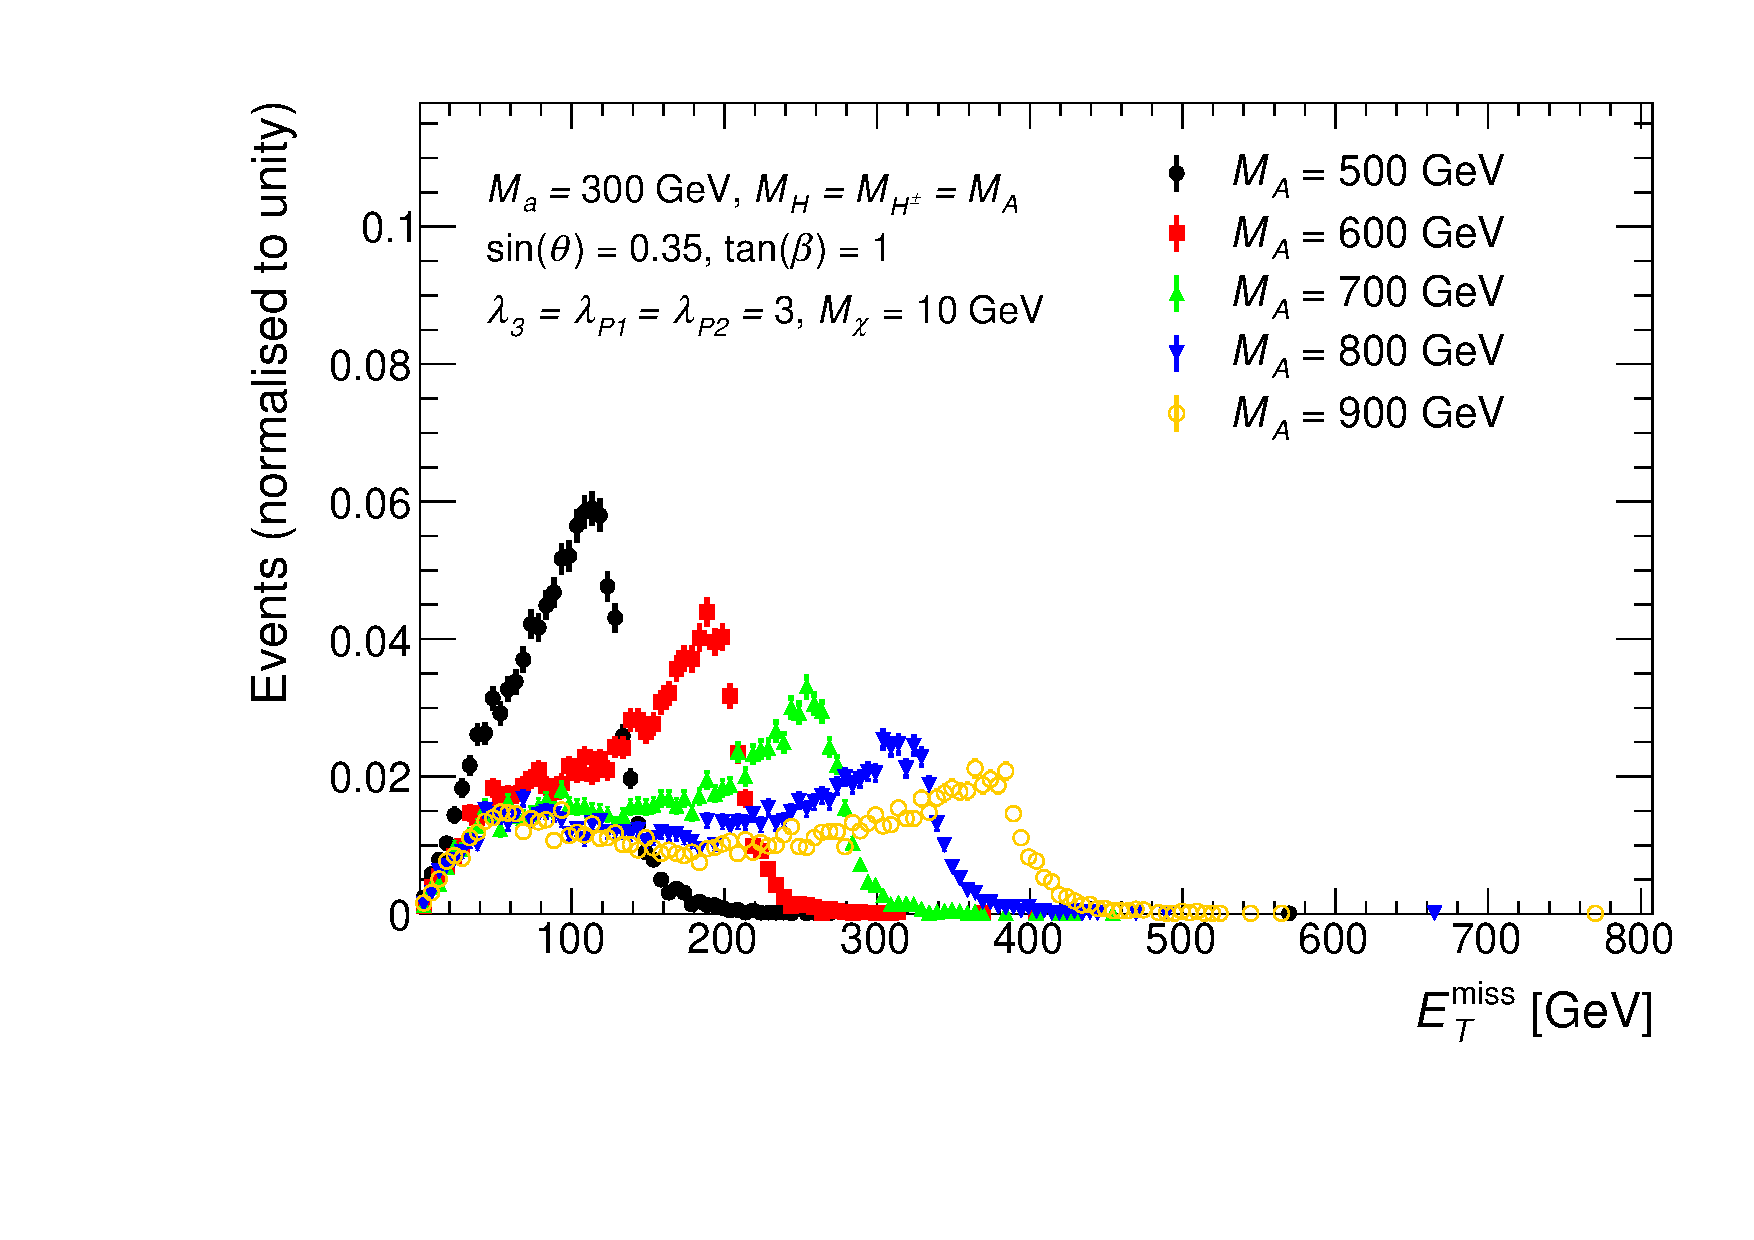
\includegraphics[width=\textwidth]{texinputs/04_grid/figures/monoHbb_m_large_A_scan_MET_liny_norm2one.pdf}
	\caption{$\MET$ distribution for points with different $\mA~(=\mH=\mHc)$
    and fixed $\ma = 300$ GeV. 
	\label{fig:monoHbb_mA_scan_met}} 
    \end{subfigure}
    \begin{subfigure}[t]{0.48\textwidth}
	\centering
	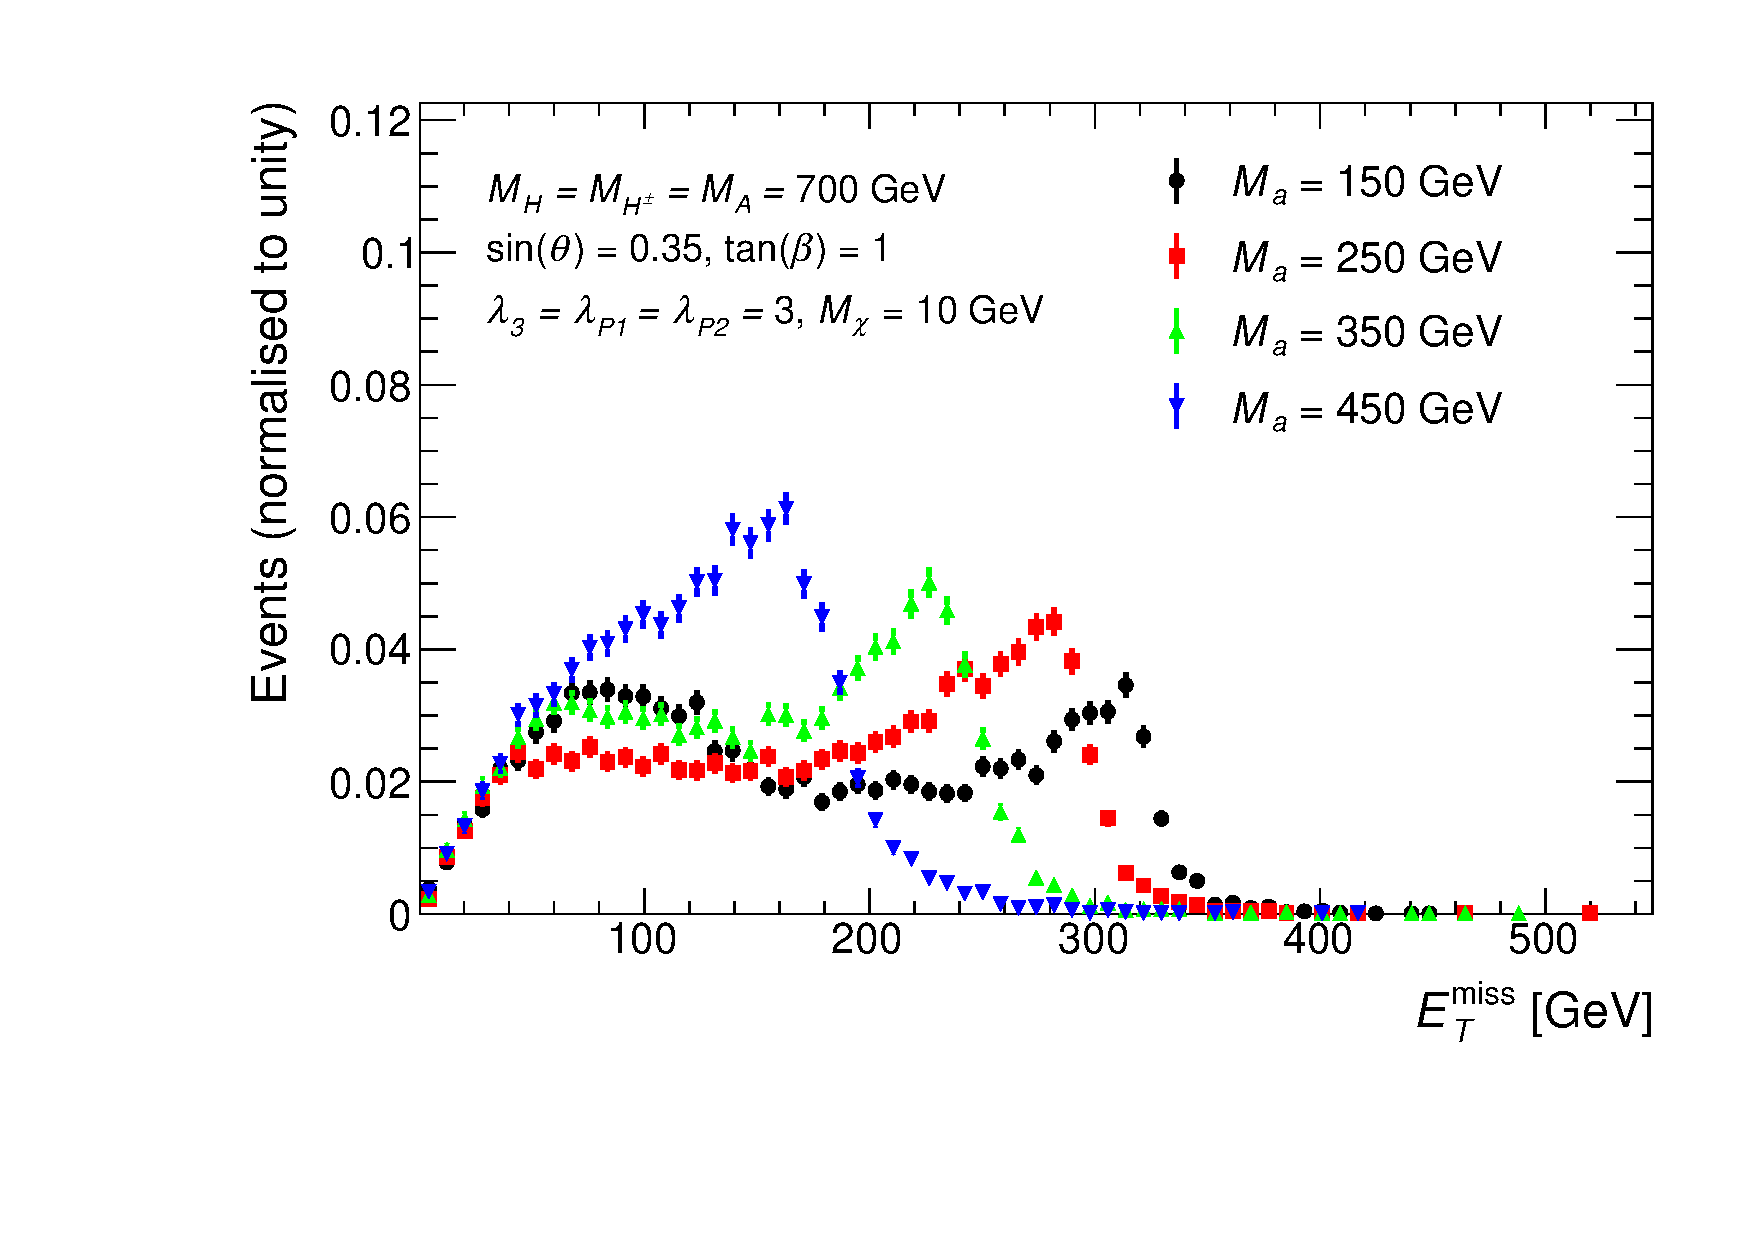
\includegraphics[width=\textwidth]{texinputs/04_grid/figures/monoHbb_m_small_a_scan_MET_liny_norm2one.pdf}	
	\caption{$\MET$ distribution for points with different $\ma$ and fixed $ \mA=\mH=\mHc= 700$ GeV. 
	\label{fig:monoHbb_ma_scan_met}}
    \end{subfigure}
    
    \caption{Parton-level $\MET$ distribution in \monohbb events for different $\ma$ and $\mA$, with $ \sinp = 0.35, \tanb = 1, \mDM = 10$ GeV and $ \lap1 = \lap2 = \lam3 = 3 $}
\end{figure}

\begin{figure}%[!htbp]
	\centering

    \begin{subfigure}[t]{0.75\textwidth}
	\centering
	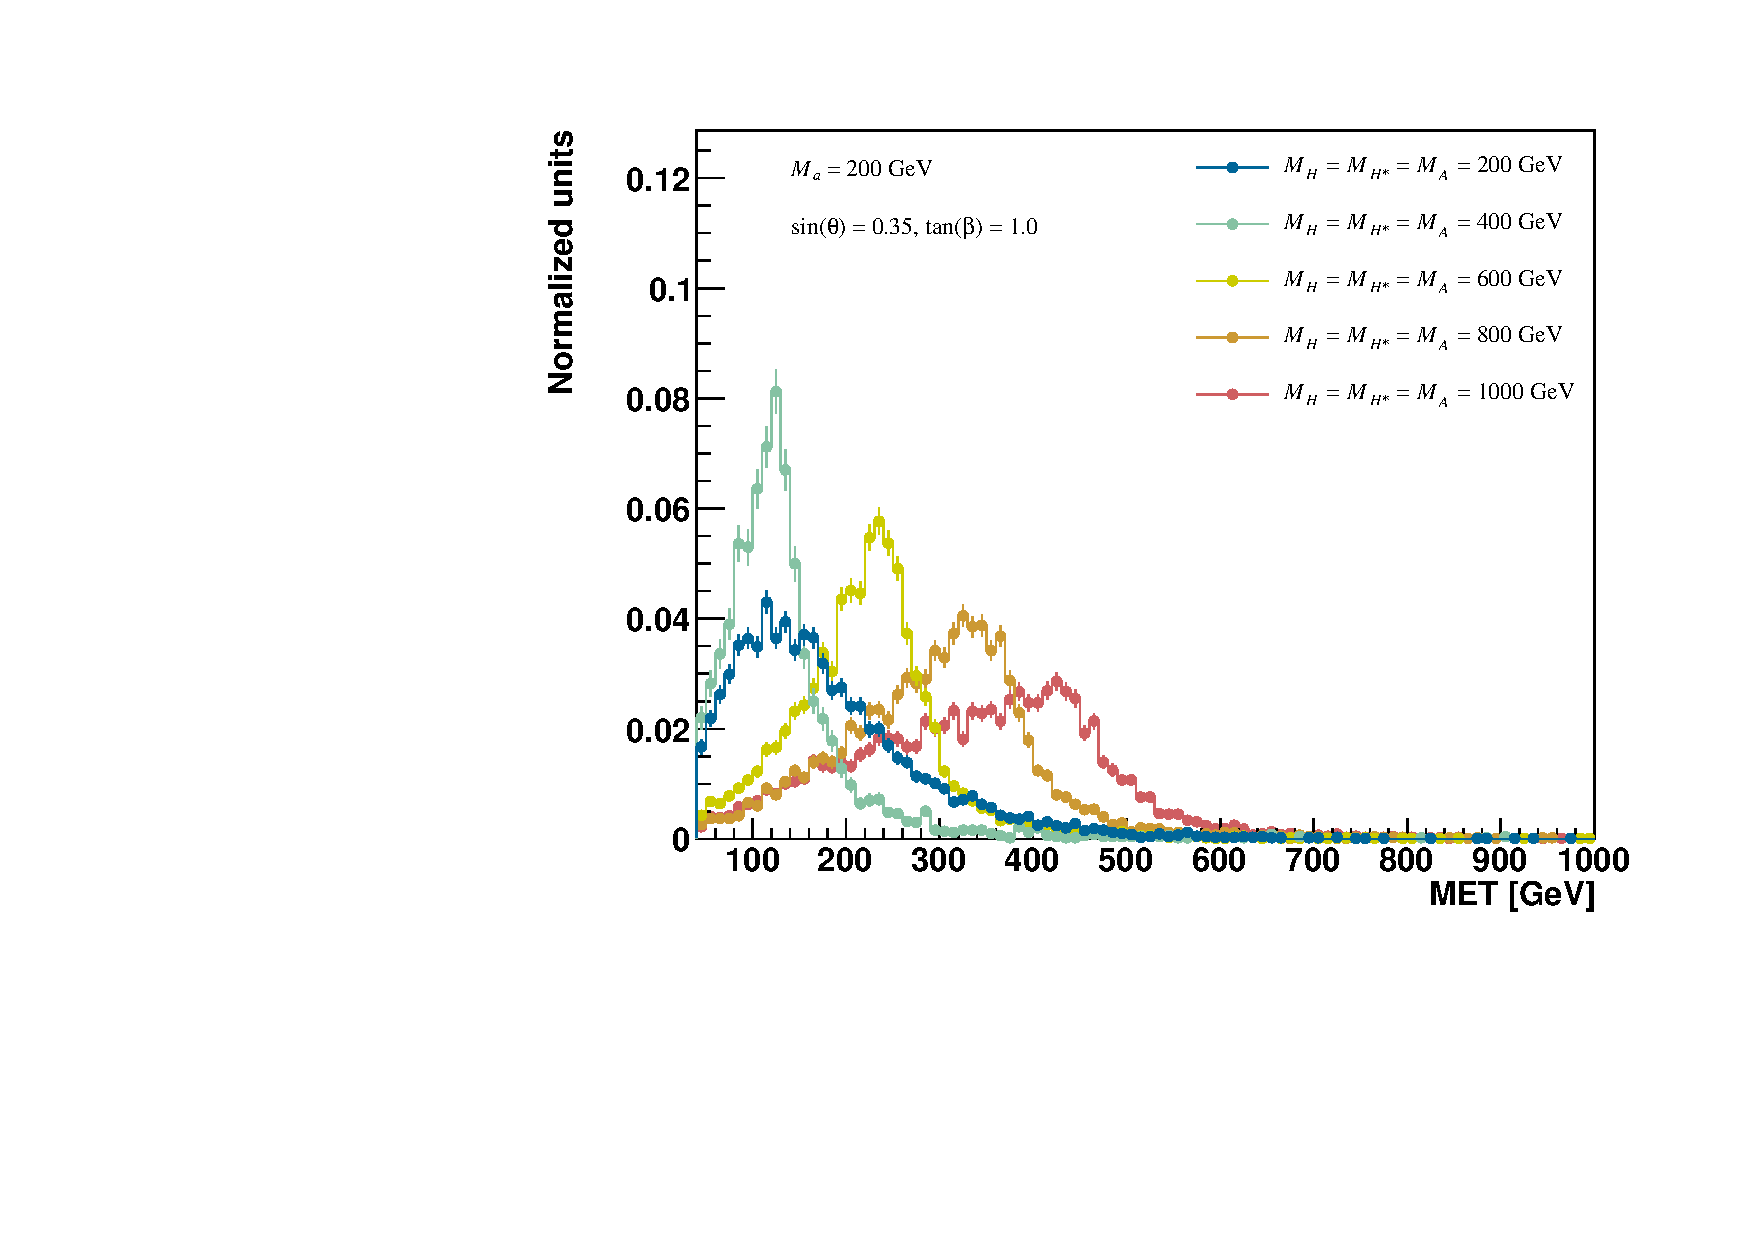
\includegraphics[width=\textwidth]{texinputs/04_grid/figures/monoz/leptonic/mAscan_for_ma200_axis.pdf}	
	\caption{The \MET distribution in signatures including a Z boson after preselection, with varying \mA values for fixed \ma = 200 GeV and \mA = \mH. \label{fig:monoz_ll_mA_scan}}
    \end{subfigure}

\end{figure}

\begin{figure}
\centering
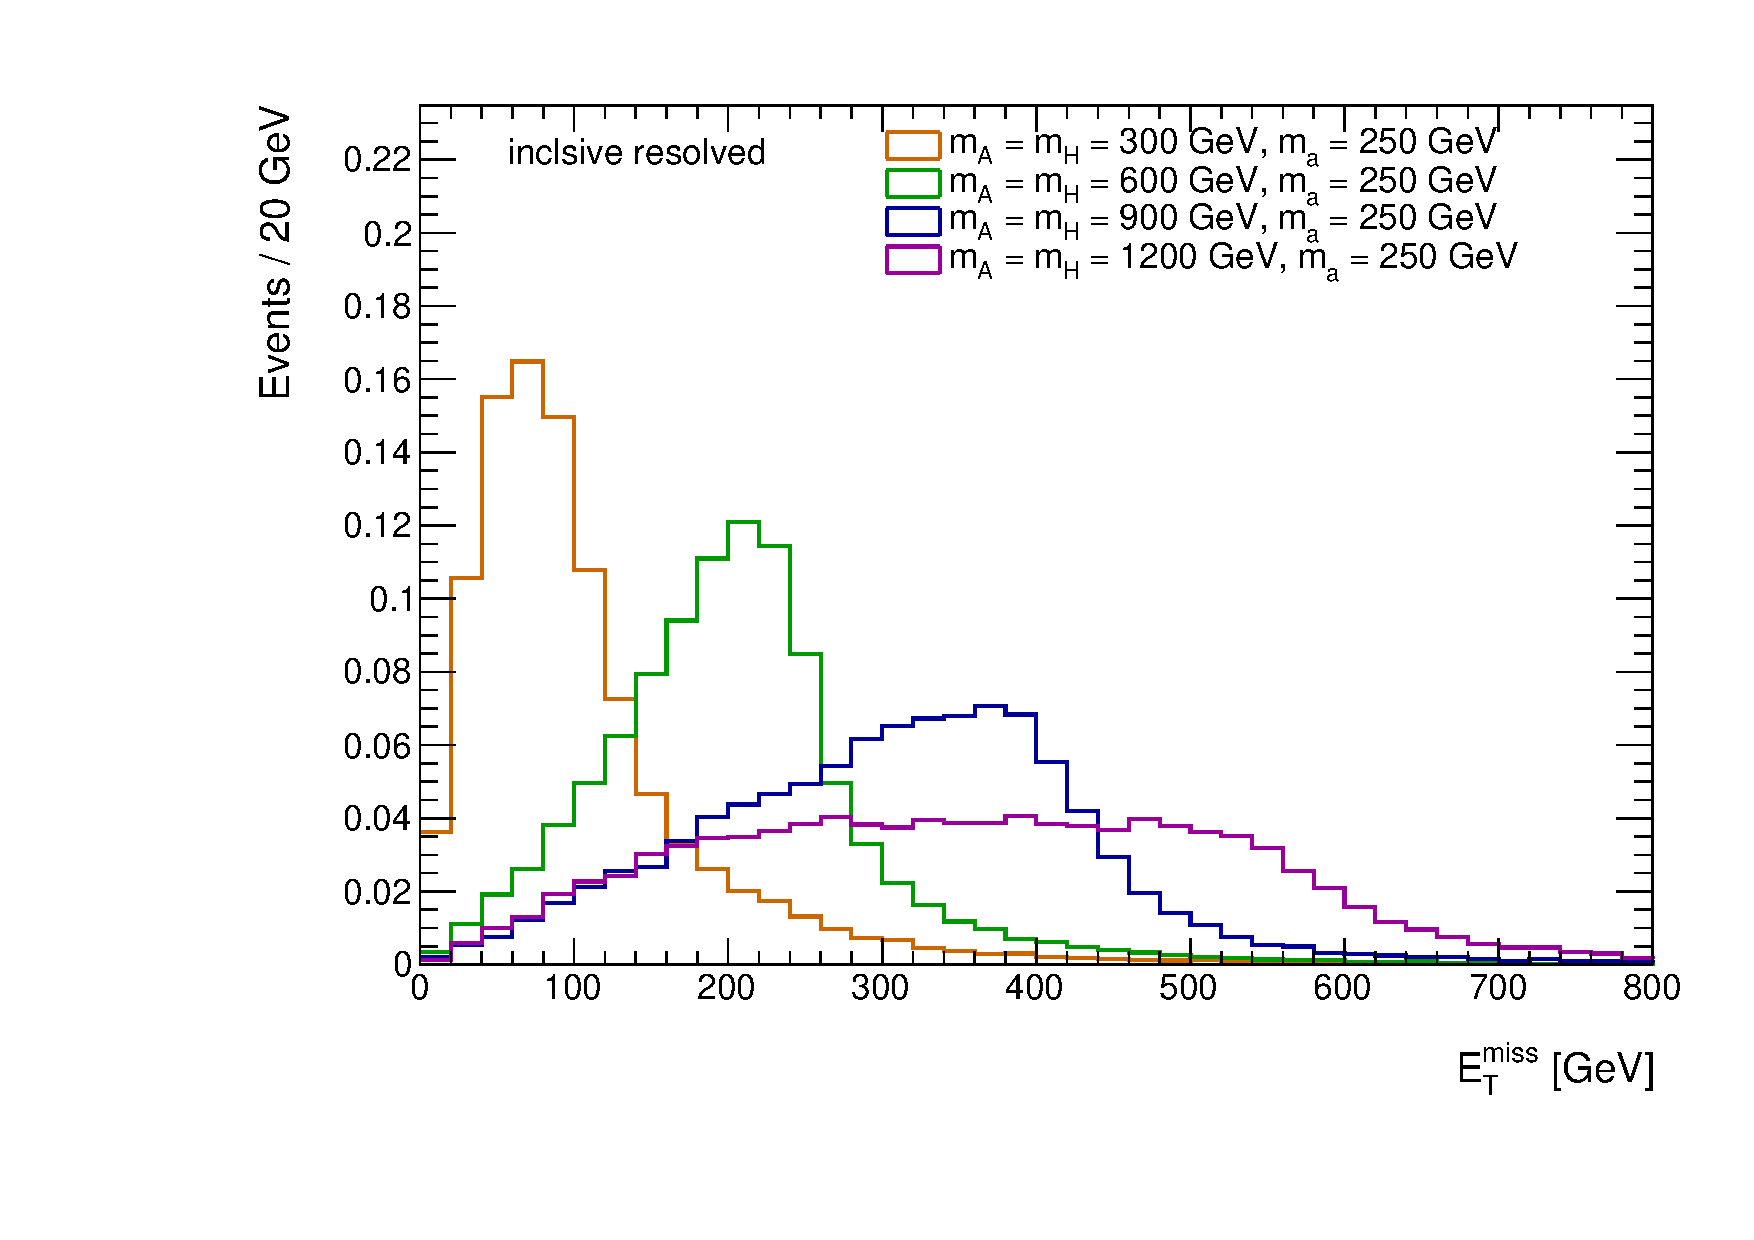
\includegraphics[width=0.45\textwidth]{texinputs/04_grid/figures/monoz/hadronic/ma250_incl_resl_MET_linear.pdf}
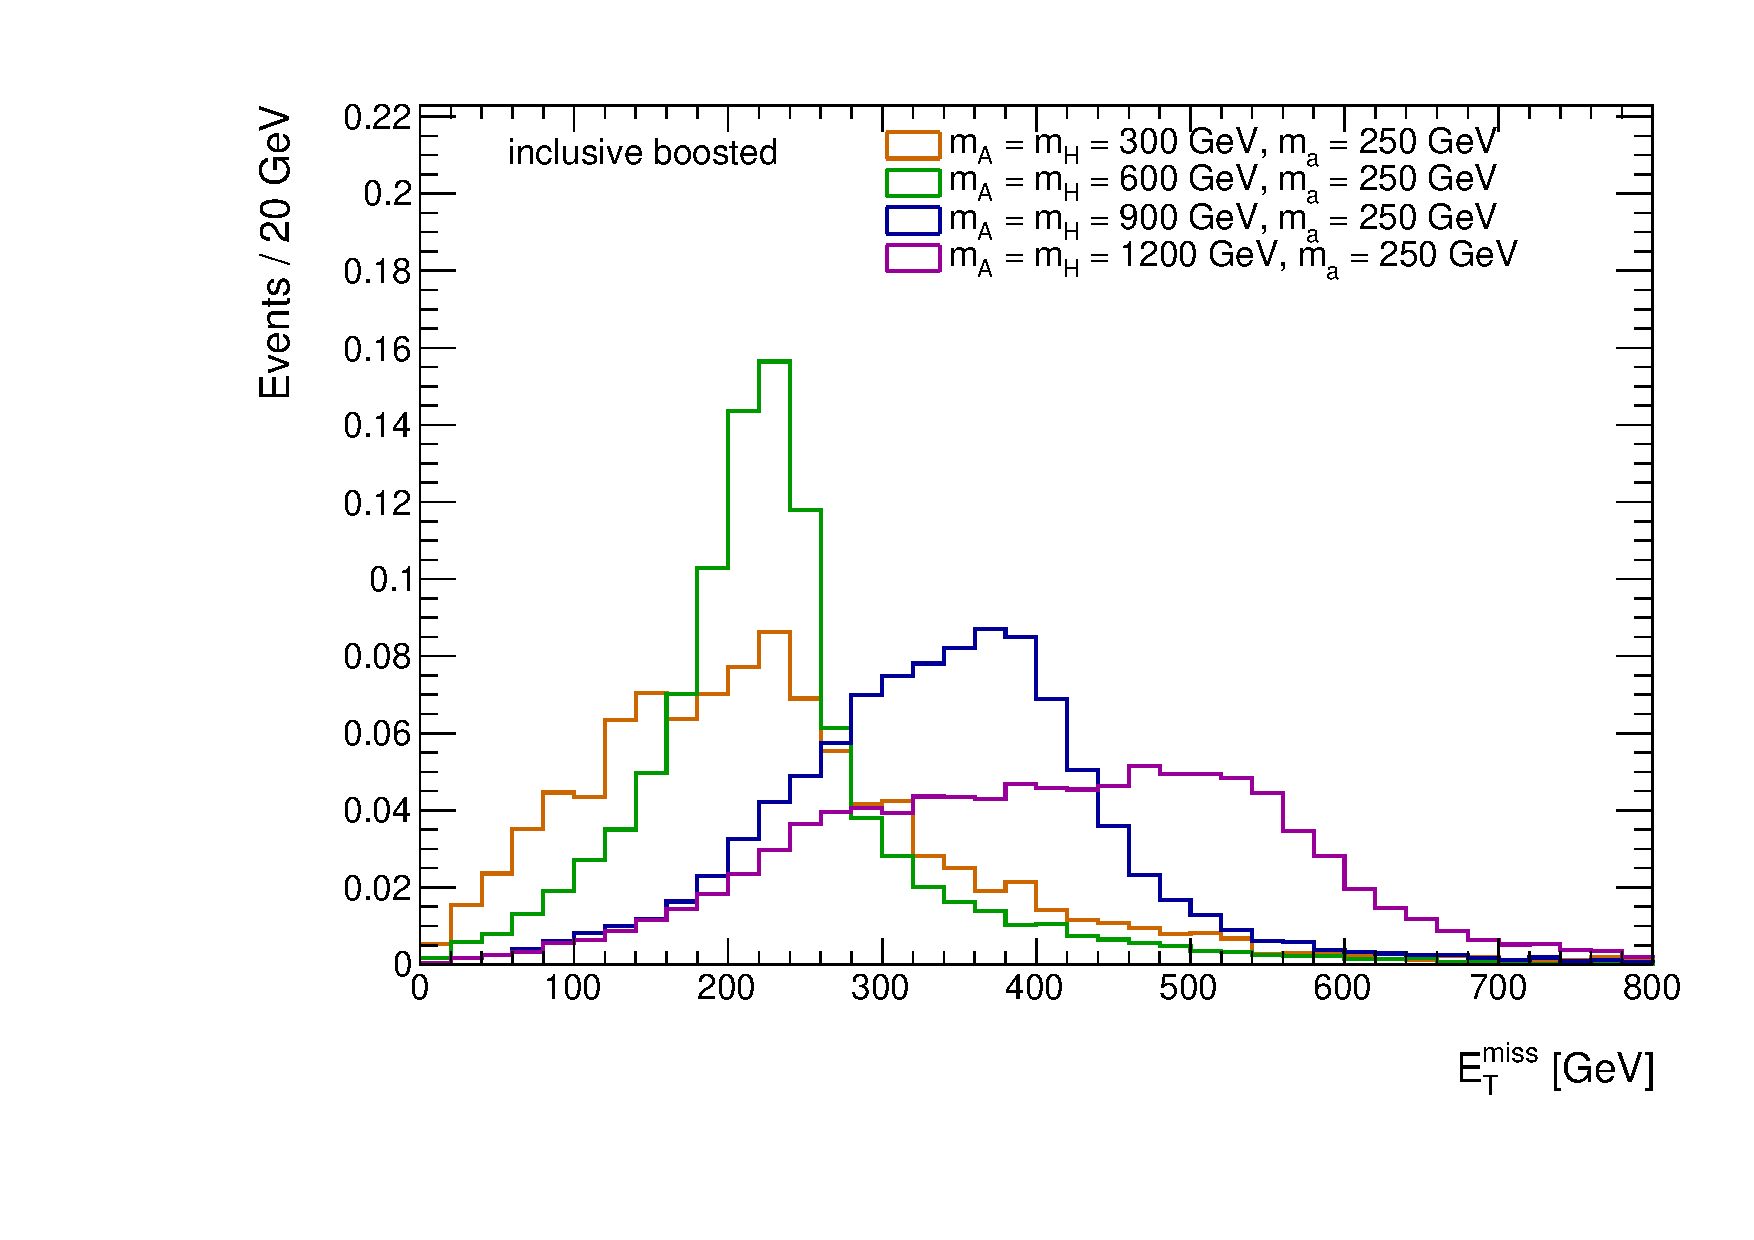
\includegraphics[width=0.45\textwidth]{texinputs/04_grid/figures/monoz/hadronic/ma250_incl_merged_MET_linear.pdf}
\caption{Dijet mass (top), $\Delta\Phi(jj, \MET)$ (middle) and $\MET$ (bottom) distributions 
after applying the inclusive selections in the resolved analysis are shown on the left side. Large-radius 
jet mass (top), $\Delta\Phi(J, \MET)$ (middle) and $\MET$ (bottom) distributions 
after applying the inclusive selections in the boosted analysis are shown on the right side. 
The signal masses are chosen to be \mA = 300, 600, 900 and 1200~GeV with the fixed \ma = 250~GeV.}
\label{fig:monozhad_kin_inc_fixed_ma}
\end{figure}

\begin{figure}
\centering
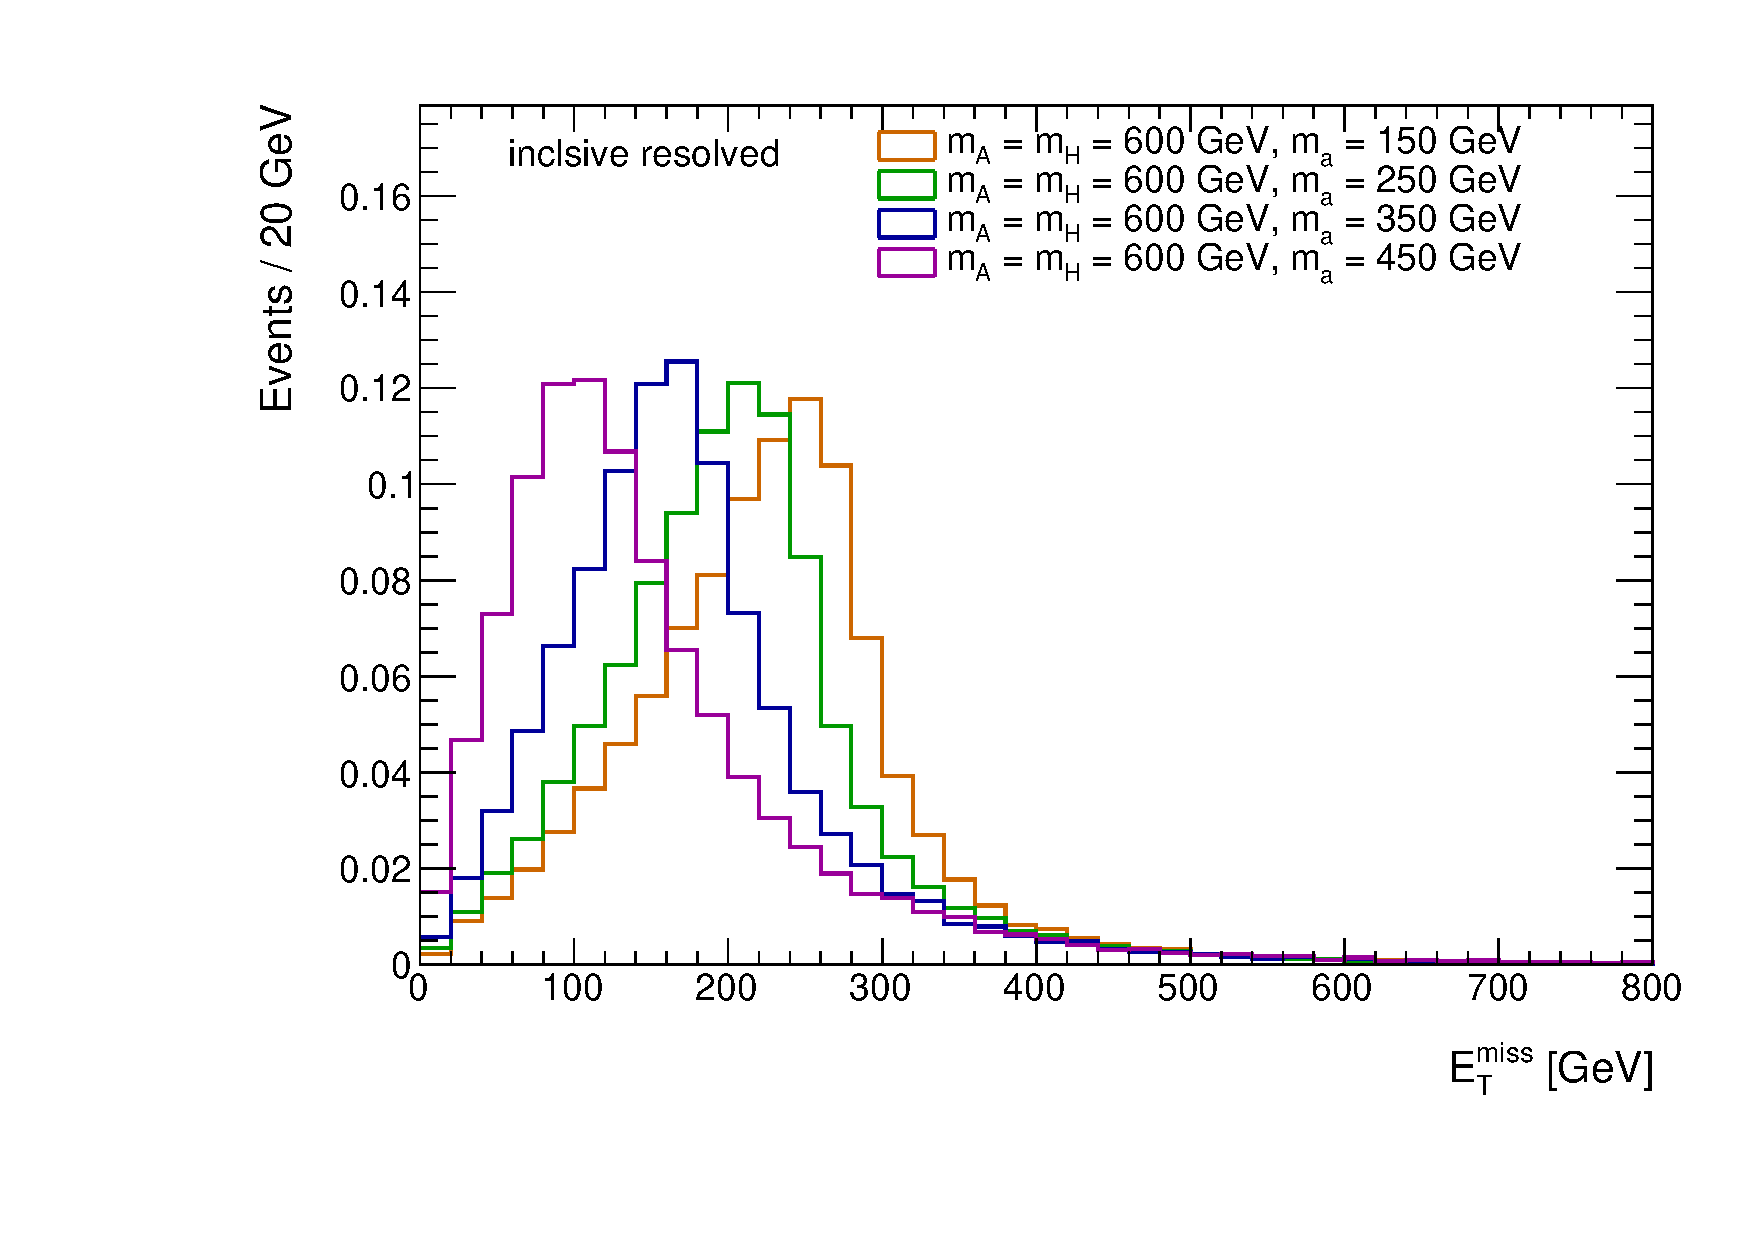
\includegraphics[width=0.45\textwidth]{texinputs/04_grid/figures/monoz/hadronic/mA600_incl_resl_MET_linear.pdf}
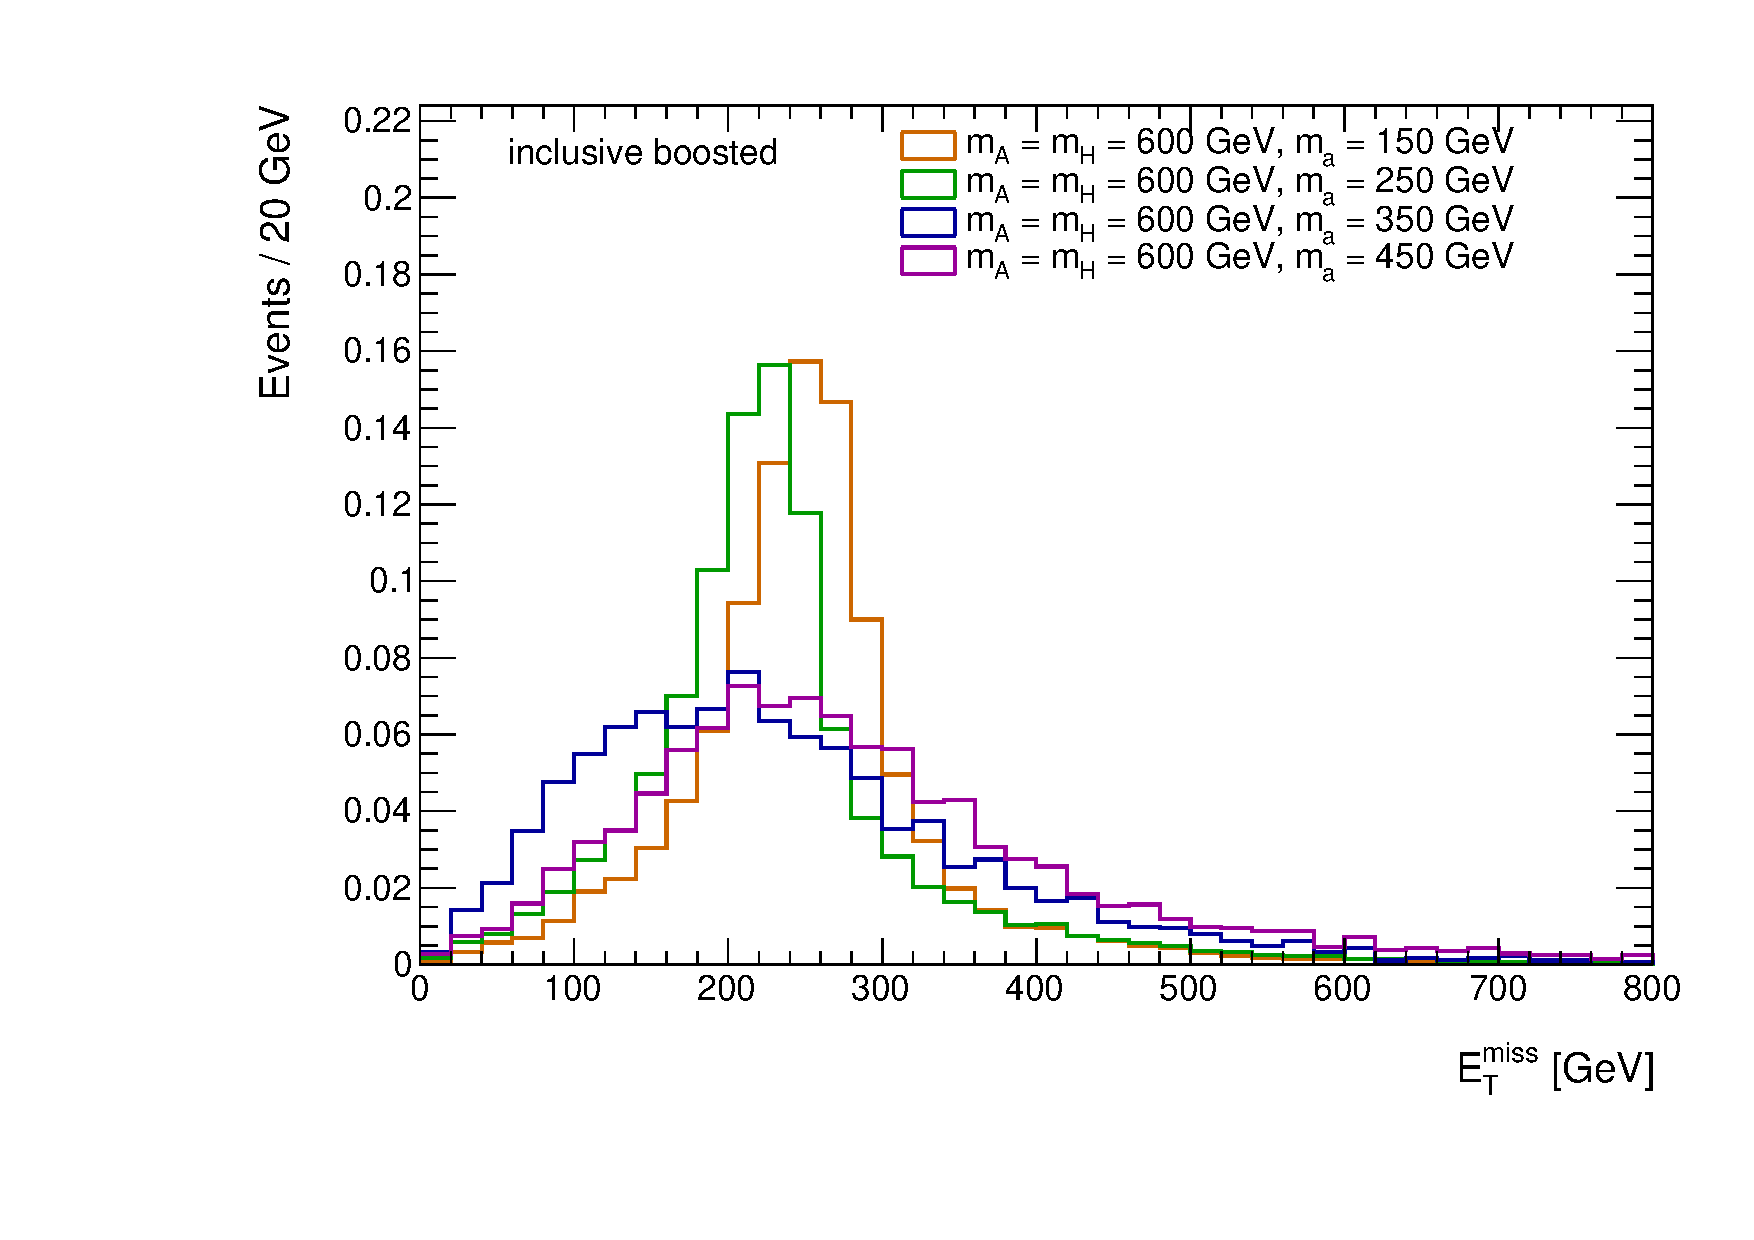
\includegraphics[width=0.45\textwidth]{texinputs/04_grid/figures/monoz/hadronic/mA600_incl_merged_MET_linear.pdf}
\caption{Z (hadronic) + \MET search $\MET$ distributions 
after applying the inclusive selections in the resolved analysis are shown on the left side, and on the right side
for the boosted analysis. The signal masses are chosen to be \ma = 150, 250, 350 and 450~GeV with the fixed \mA = 600~GeV.}
\label{fig:monozhad_kin_inc_fixed_mA}
\end{figure}

Some fraction of signal events is also produced in non-resonant $2 \to 3$ processes $gg \to h \chi \chi$, as in \autoref{fig:feyn_hdm_box}, leading to a broader distribution of the invariant mass of the decay products.  
%link into thereory section graph or cite paper
Consequently, this results in a broader and softer \met distribution that is distinct from the Jacobian peak discussed above, and contributes to the off-peak features of \autoref{fig:monoHbb_ma_scan_met} and \autoref{fig:monoHbb_mA_scan_met}. 

Since the shape of the $\MET$ distribution affects the design of experimental searches, and to a large extent their sensitivity, it is recommended to scan the $\mA$ and $\ma$ parameter space. 

%In conclusion, the $\mA$ and $\ma$ parameters strongly affect the sensitivity of a search for the \hdma model using the \monohbb signature because they determine the location of the Jacobian peak in the \met distribution. Therefore, one of the proposed parameter scans for the \hdma model is in the ($\ma$,$\mA$) plane.

\begin{figure}%[!htpb]
\centering
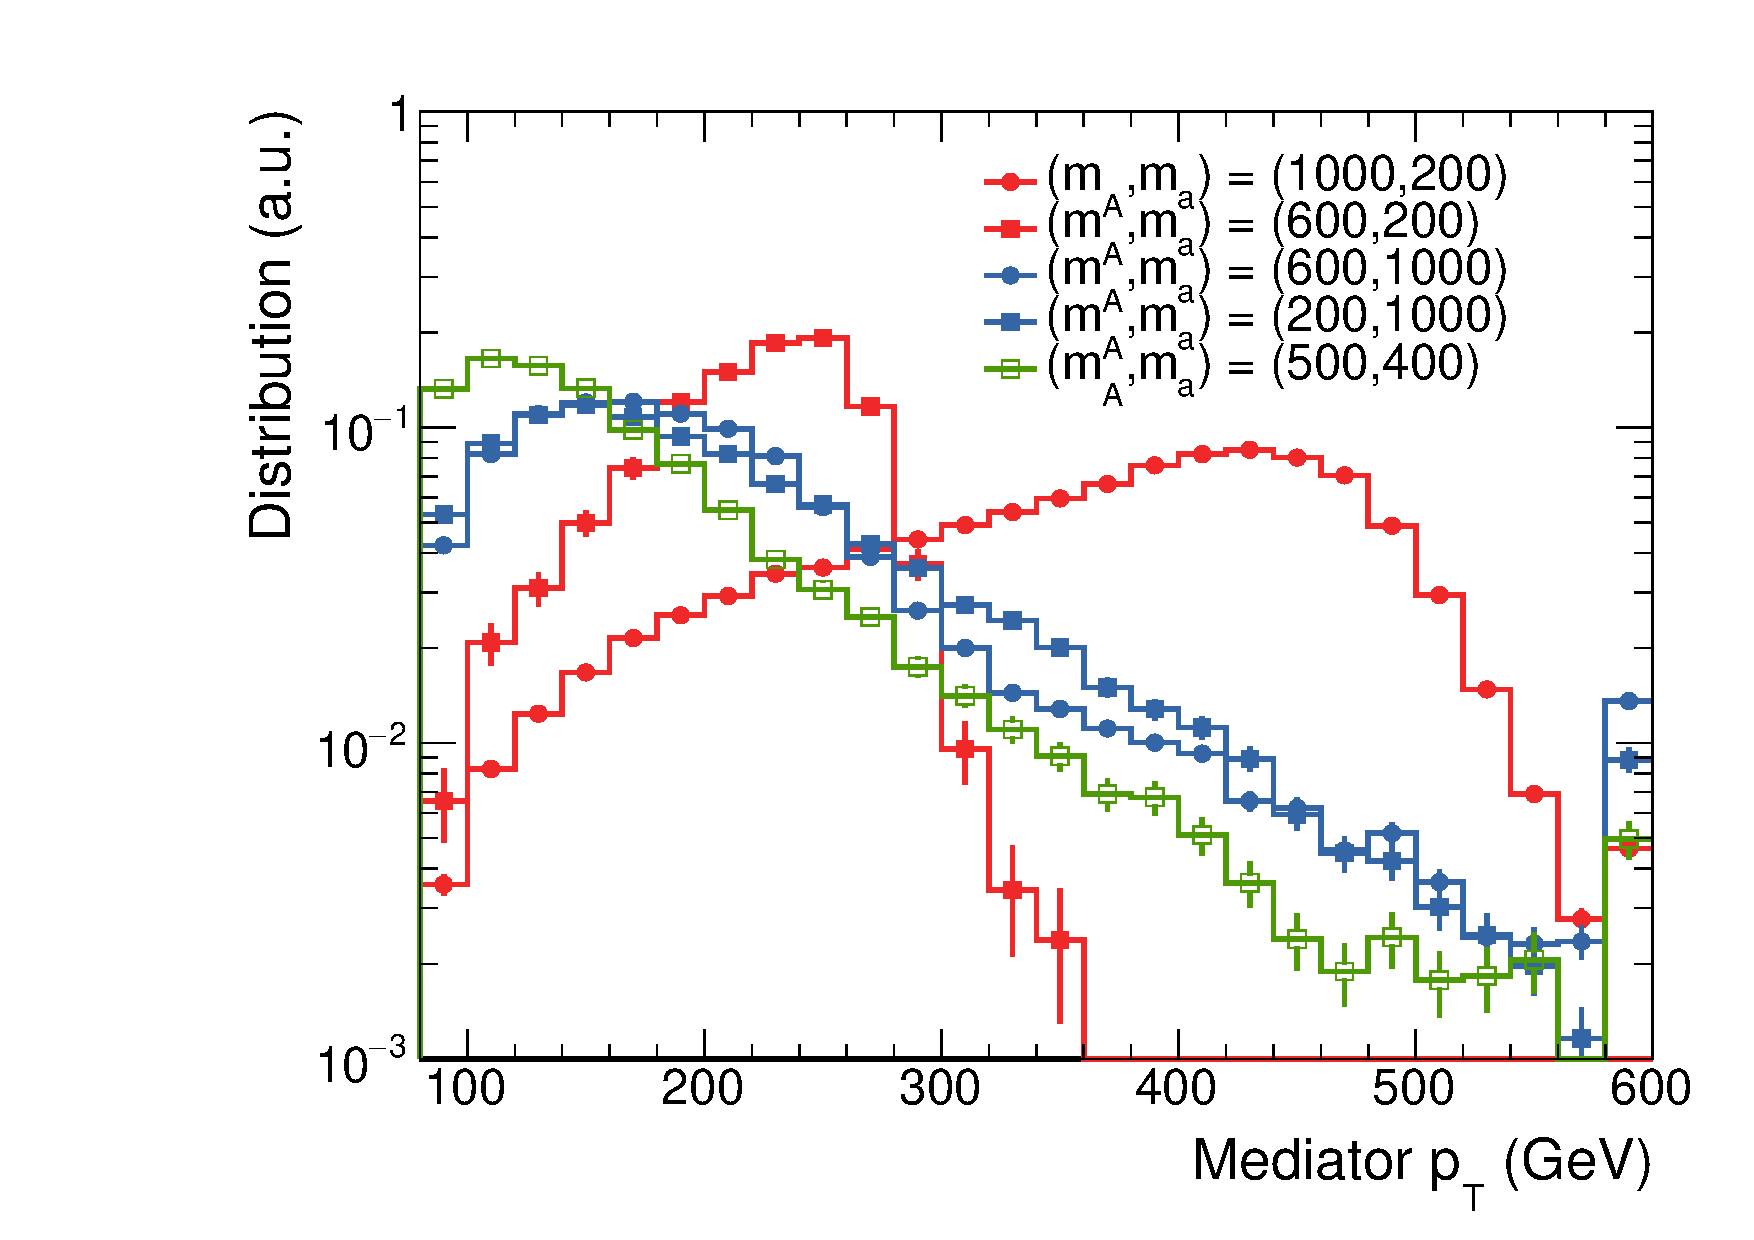
\includegraphics[width=0.45\textwidth]{texinputs/04_grid/figures/monoz/leptonic/dmwg-final_h_pt_med_dm.pdf}
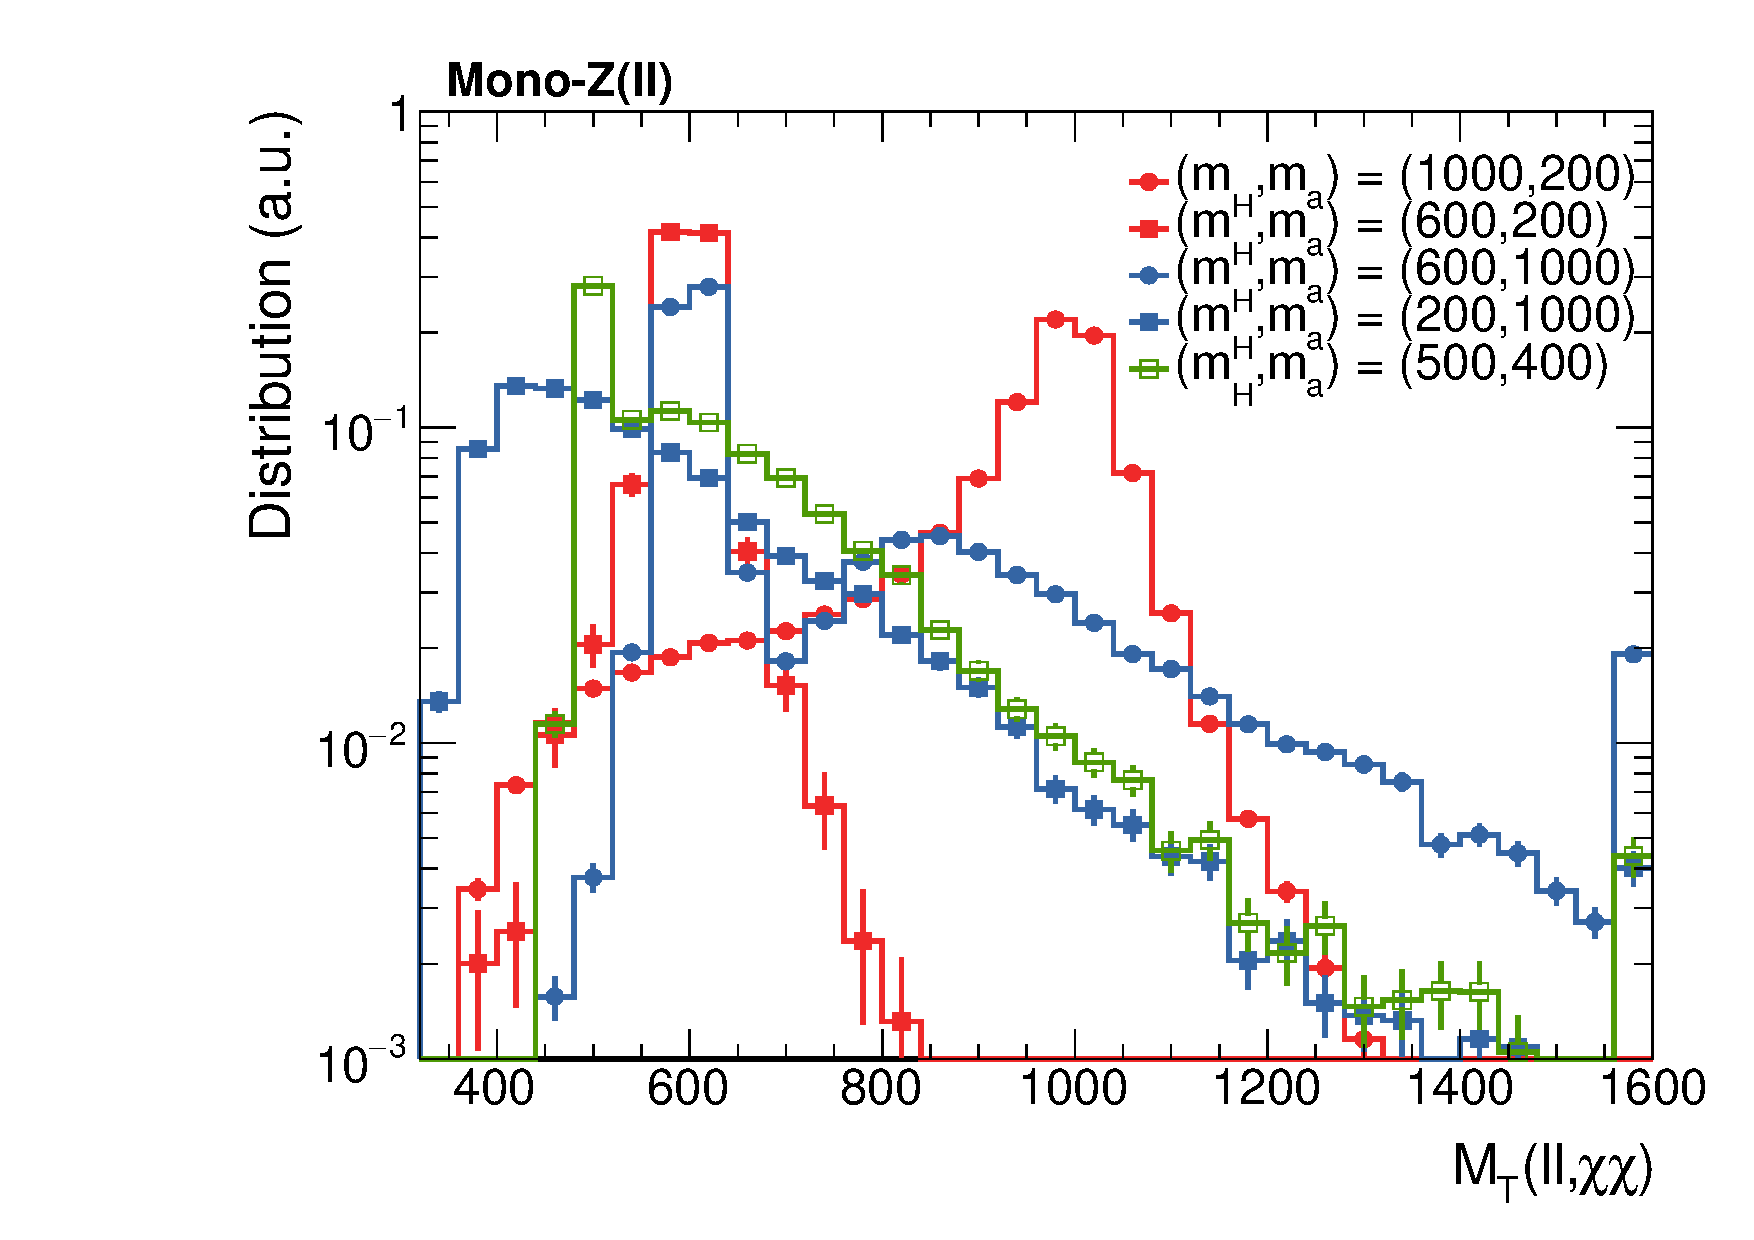
\includegraphics[width=0.45\textwidth]{texinputs/04_grid/figures/monoz/leptonic/dmwg-final_h_mt_total.pdf}
\caption{\MET and  $\MT$ distributions after the full selection of Z(lep)+\MET search. Both distributions show a peaked structure around $\mA$ in the $\mA > \ma$ regime, reflecting the resonant production of $A$.}
\label{fig:monoz_kin_final}
\end{figure}

As an additional remark on the design of these searches, the distributions of the $\MET$ and $\MT$ variables after final selection are shown in ~\autoref{fig:monoz_kin_final} for the Z+\MET searches. Traditionally, these searches have relied on the $\MET$ distribution for signal extraction. While the presence of the Jacobian peak structure in the distribution facilitates signal-background separation, it may be beneficial to also consider the $\MT$ distribution. Although only transverse information is available, the resonant structure of the signal is significantly enhanced in the $\MT$ variable, which may enhance the sensitivity of a specialized search strategy exploiting this characteristic.
In the region of inverted mass hierarchy $\mA < \ma$, the \MET spectrum is less structured and does not fall off as steeply towards higher values. For a small mass splitting of $\ma-\mA\approx M_{Z}$, the spectrum is shifted to much lower values of \MET. 
The $\MT$ distribution allows to access the resonant nature of the process. Clear mass peaks are present for the normal mass hierarchy. In the inverted region, the MT distribution is more sensitive to the mass difference $\ma-\mA$ than the \MET distribution, allowing to differentiate between signal hypotheses that give near-identical \MET distributions.

\subsubsection{Masses of the heavy neutral and charged scalar Higgs bosons $H, H^{\pm}$ ($\mH$, $m_{H^{\pm}}$)}

The mass of the heavy neutral scalar Higgs boson $H$ has an indirect effect on the rate and kinematics of the signal. 
This is caused by the dependence of the coupling strengths and thus decay widths of  the pseudoscalars $A$ and $a$ on  $\mH$~\cite{Bauer:2017ota}. 
Therefore, a change of $\mH$ can affect the relative contribution of resonant versus non-resonant signal processes, as illustrated in \autoref{fig:monoHbb_mH_scan_met}.

The choice $\mH = \mA$ results in a detectable total cross section for many signal points and a dominant contribution of the resonant signal process. 
%Do we show this somewhere?
This choice allows us to test diverse $\MET$ distributions and results in about equal contributions to the sensitivity through the \monoz and \monoh signatures, highlighting their complementarity. For this reason $\mH = \mA$ is adopted for all scans. For simplicity, the neutral scalar $H^{\pm}$ is assumed to be mass-degenerate to $H$, as it does not affect the \hdma model kinematics.

%as demonstrated in \autoref{fig:monoHbb_mA_scan_met} and \autoref{fig:monoHbb_ma_scan_met}

\begin{figure}[!htbp]
	\centering

%	\begin{subfigure}[t]{0.75\textwidth}
%	\centering
	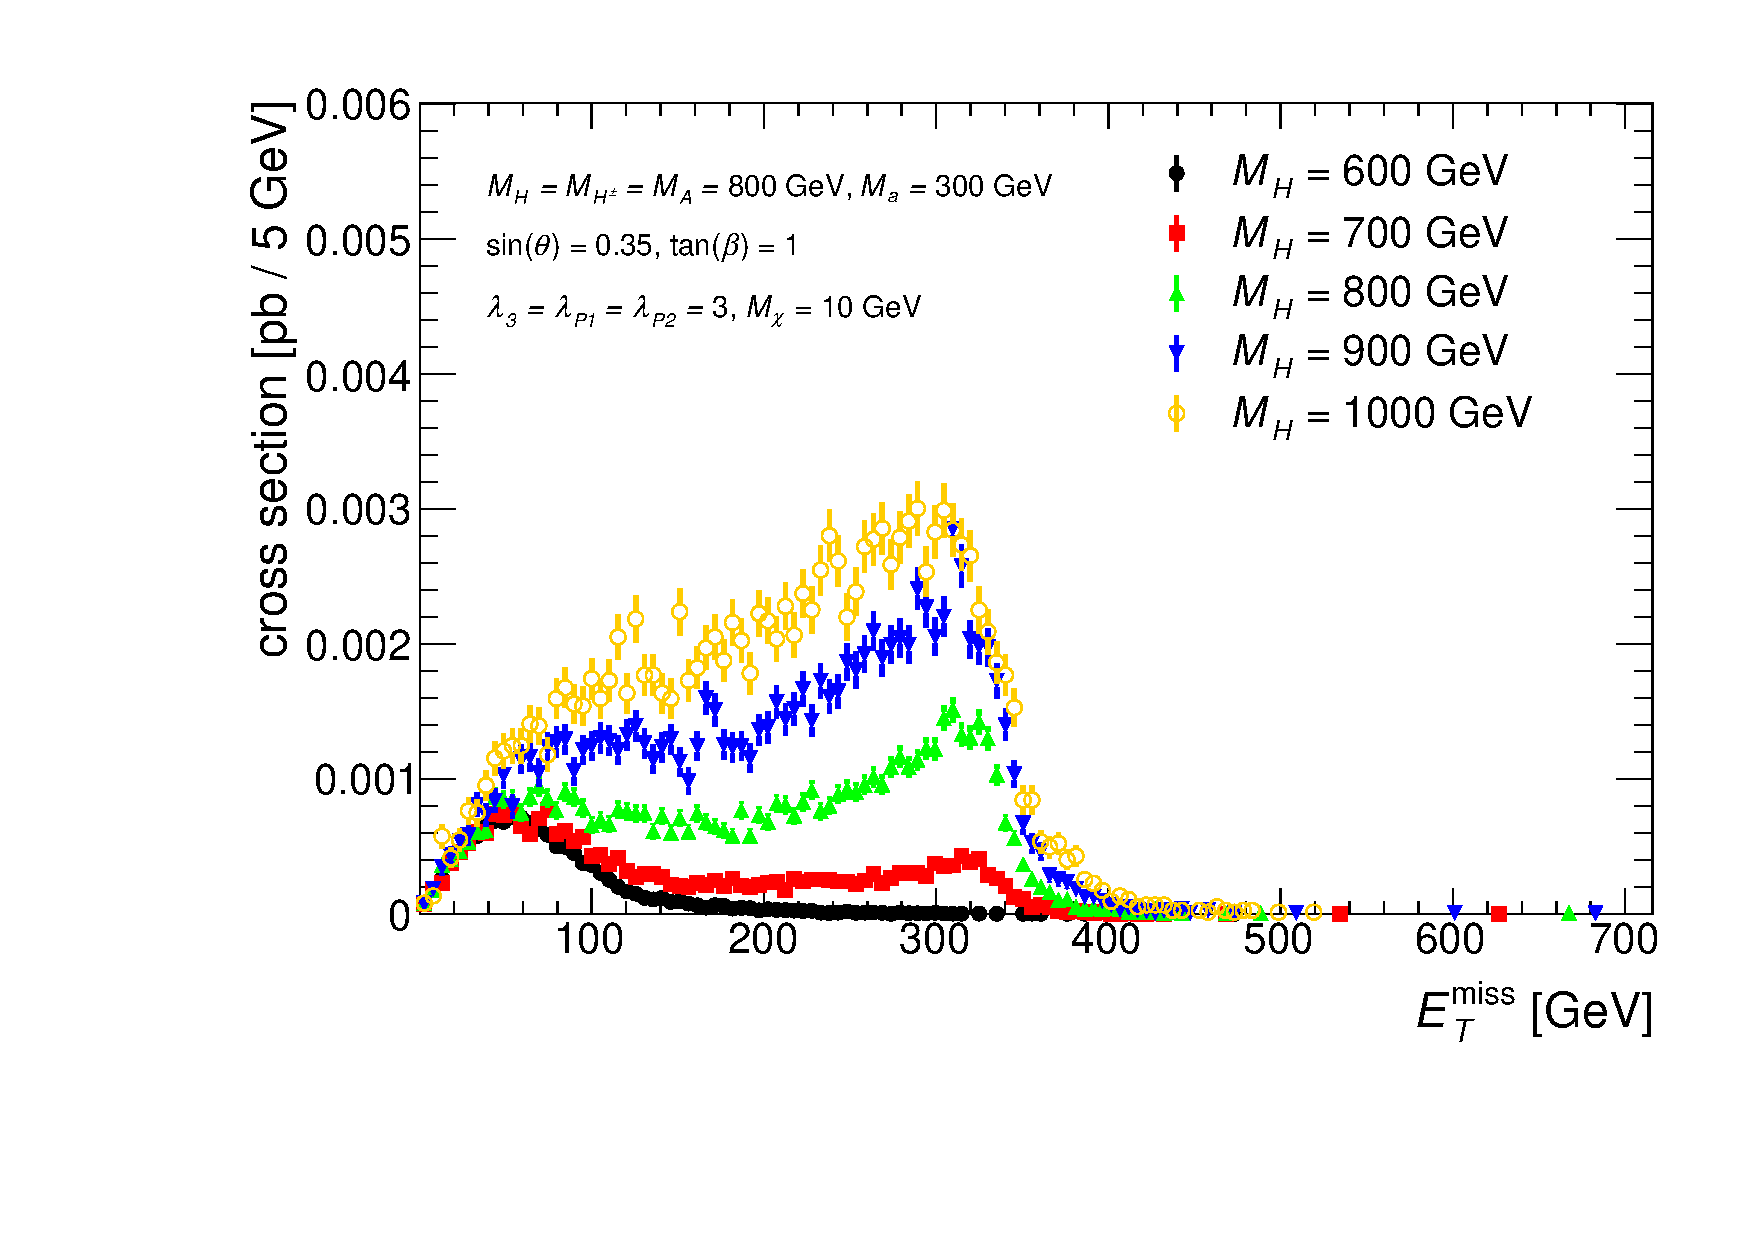
\includegraphics[width=0.75\textwidth]{texinputs/04_grid/figures/monoHbb_mH_scan_MET_liny.pdf}
	\caption{The \MET distribution, accounting for the production cross section, of \monohbb signal events for five representative choices of $\mH = \mHc$.
	%and fixed $ \mA=800$ GeV, $\ma = 300 $ GeV,  $ \sinp = 0.35, \tanb = 1, \mDM = 10$ GeV and $ \lap1 = \lap2 = \lam3 = 3 $.
	\label{fig:monoHbb_mH_scan_met}} 
%    \end{subfigure}
     
	\caption{$\MET$ distribution in \monohbb and Z+\MET events for different $\mH$}
\end{figure}

\subsubsection{Mixing angle between the two pseudoscalars $A$ and $a$ ($\sinp$)}

The sine of the mixing angle between the two pseudoscalars $A$ and $a$, $\sinp$,affects not only the cross section, but also the shape of the \MET\ distribution in searches including a Higgs boson, as shown in \autoref{fig:monoHbb_sinp_scan_mA600_ma200_met}. 
For the resonant diagram $gg\rightarrow A \rightarrow ah \rightarrow \chi\bar{\chi}h$, the product of cross section times branching ratios  ${\cal B}(A\rightarrow ah){\cal B}(a \rightarrow \chi\bar{\chi})$ scales with $\sin^2\theta\cos^6\theta$, while for the diagram $gg\rightarrow a \rightarrow A^*h \rightarrow \chi\bar{\chi}h$, the product of cross section times branching ratios ${\cal B}(a\rightarrow Ah){\cal B}(A \rightarrow \chi\bar{\chi})$ scales with $\sin^6\theta\cos^2\theta$. 
Therefore, at small \sinp, the resonant diagram $A\rightarrow ah$ is the dominant production mode and the \MET\ distribution has a Jacobian peak following \autoref{eq:monoH_peak_met}; while at large \sinp, the $a\rightarrow A^*h$ diagram starts to dominate and produces a second peak at a lower \MET\ value.
Scans of the \sinp parameter show they have minimal effect on the kinematic distributions for searches with a Z boson (\autoref{fig:monoz_kin_sintheta}).  

\begin{figure}%[!htbp]
	\centering

	\begin{subfigure}[t]{0.75\textwidth}
	\centering
	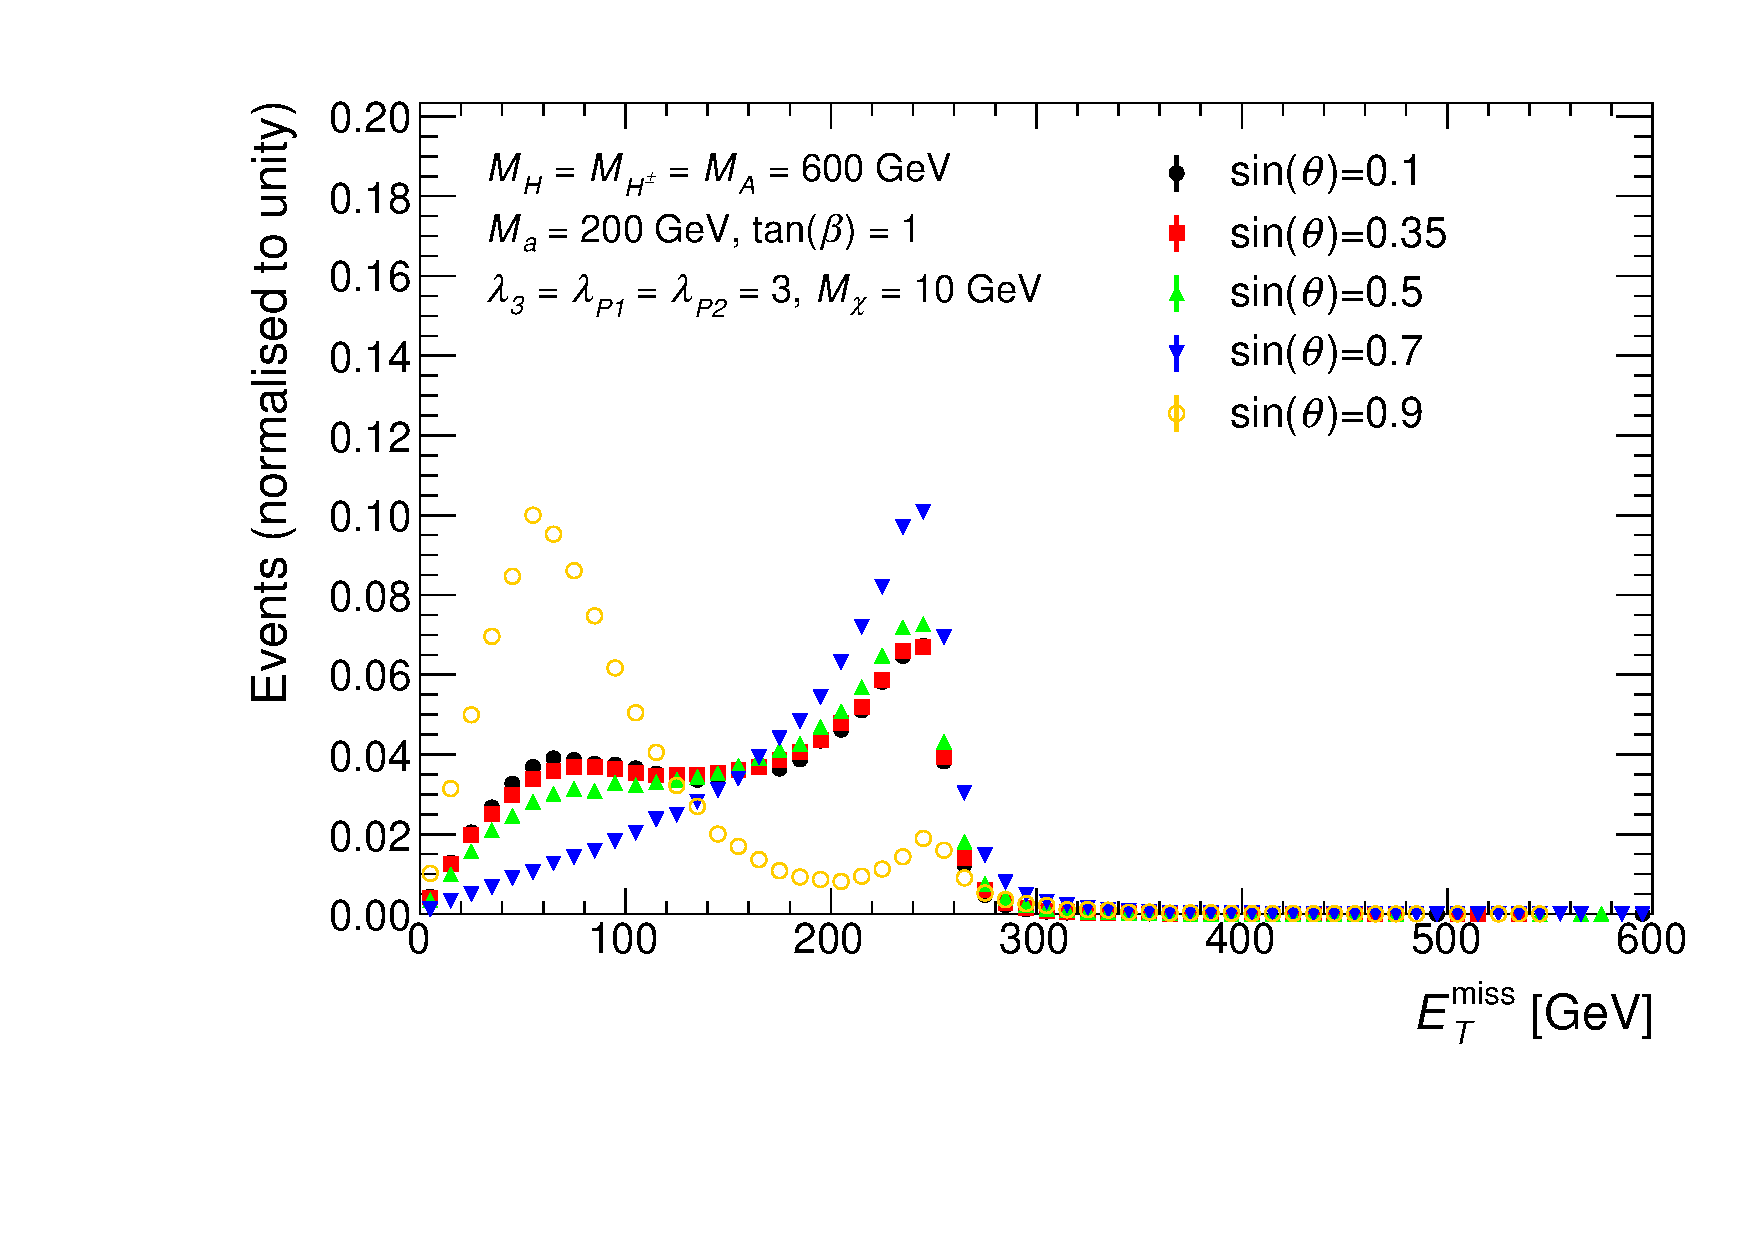
\includegraphics[width=\textwidth]{texinputs/04_grid/figures/monoHbb_sinp_scan_MA600_Ma200_MET_liny_norm2one.pdf}
	\caption{$\MET$ distribution for for five representative models with different $\sinp$ and fixed $\mA = \mH = \mHc = 600 $~GeV, $\ma = 200$~GeV.
	\label{fig:monoHbb_sinp_scan_mA600_ma200_met}} 
    \end{subfigure}
    \begin{subfigure}[t]{0.75\textwidth}
	\centering
	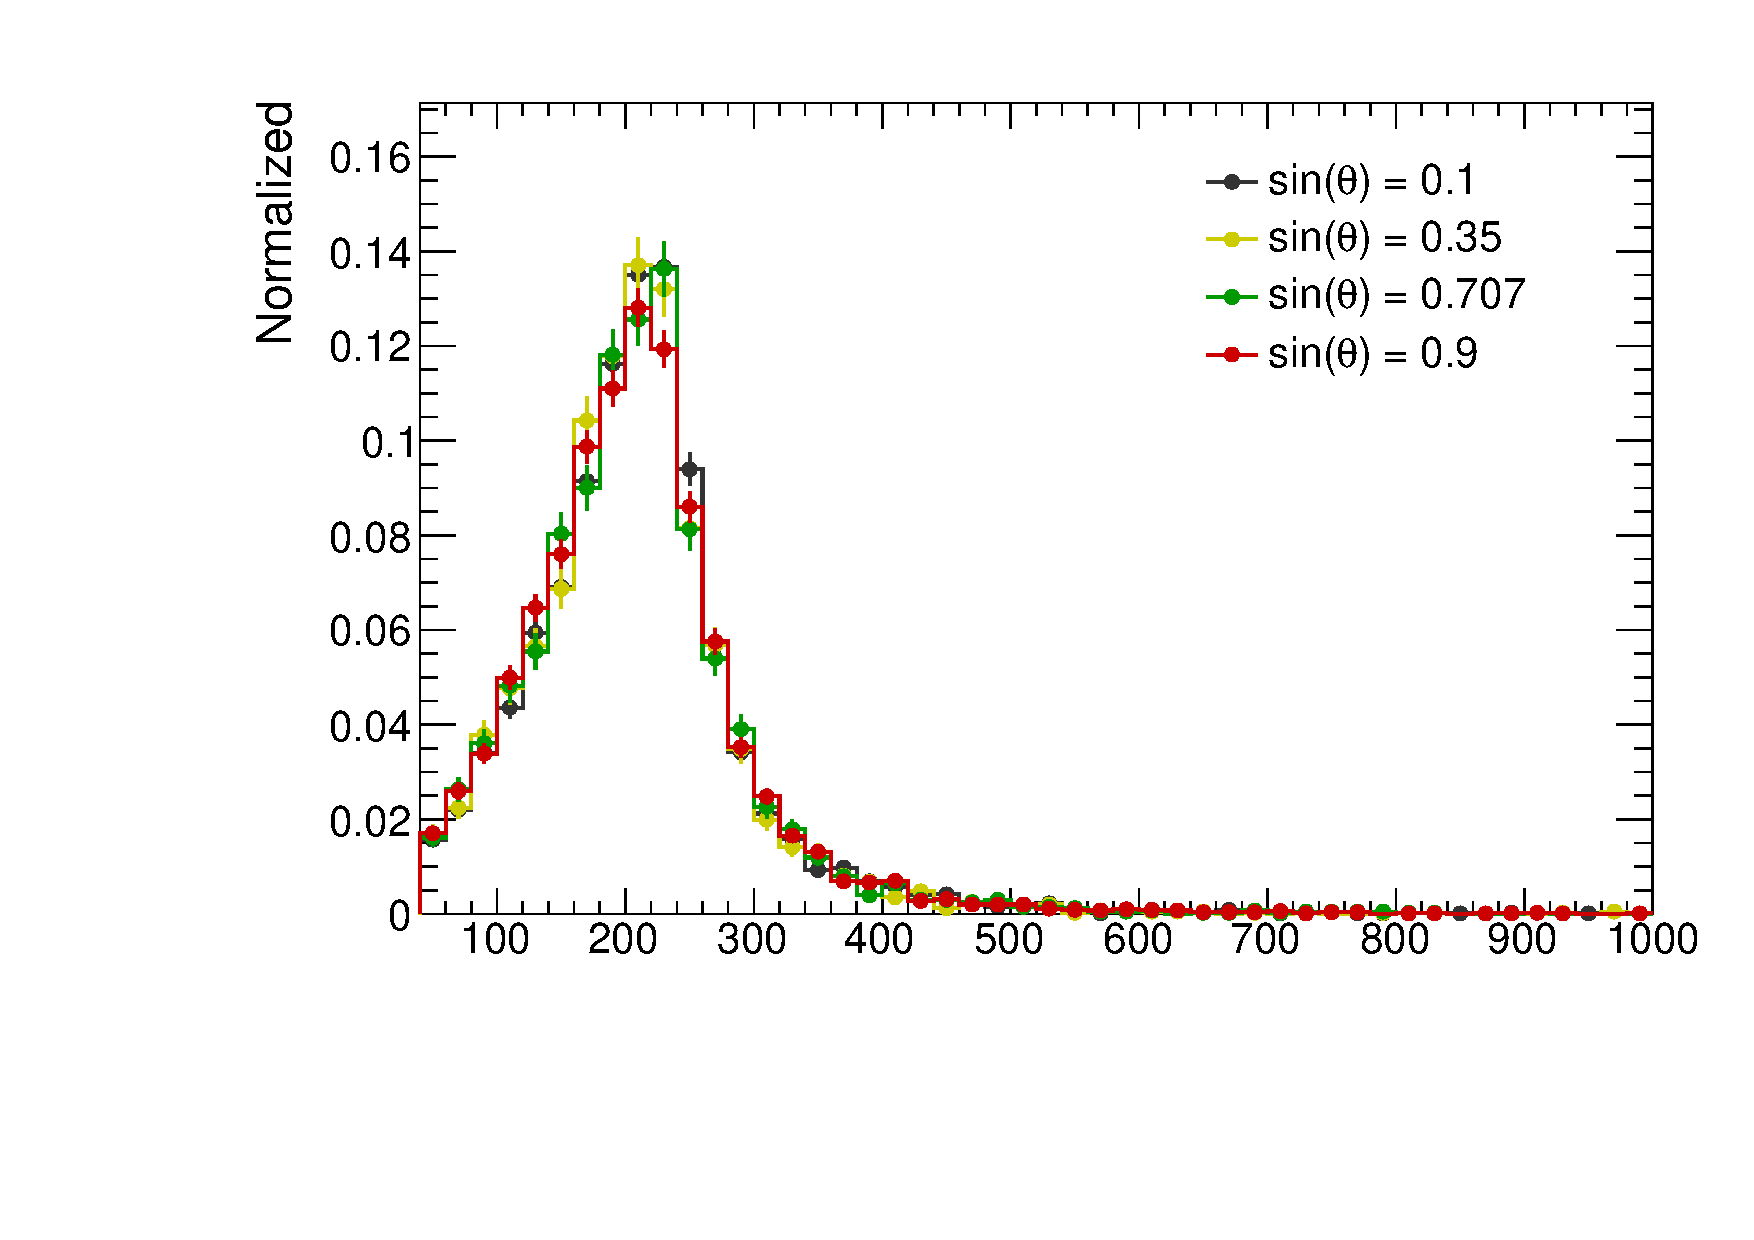
\includegraphics[width=\textwidth]{texinputs/04_grid/figures/monoz/leptonic/SinpScan_mA600_ma250_MET.pdf}	
	\caption{\MET distribution after preselection for scans of $\sin{\theta}$ for fixed $\mA = \mH = \mHc = 600 $~GeV and \ma = 250.
	\label{fig:monoz_kin_sintheta}}
    \end{subfigure}
    
    \caption{$\MET$ distributions in \monohbb and Z(lep)+\MET events for different $\sin{\theta}$. In both cases, $\tanb = 1$ and $\mDM = 10$~GeV. }
    
\end{figure}

In the \monohbb case, the shape of the $\MET$ distribution does not change much  for $\sinp < 0.7$, then changes significantly for $\sinp\geq 0.7$. 
When $\sinp=0.9$, the diagram $gg\rightarrow a\rightarrow A^*h \rightarrow \chi \bar{\chi} h$, producing a \MET peak at around 60~GeV, starts to dominate.
In the Z case, this parameter has little impact on the kinematic distributions.

\subsubsection{Ratio of the doublet vacuum expectation values ($\tanb$)}

%%% text related to tanbeta-ma scan
The shape of \MET\ distribution also has a non-trivial dependence on \tanb, as can be seen in \autoref{fig:monoHbb_tanb_scan_met}.
As discussed in the sensitivity study later, at small \tanb, the Yukawa coupling to top quark is large and the signal production mode is dominated by the non-resonant 3-body processes $gg\rightarrow h\chi\bar{\chi}$, which gives a broad and soft \MET\ spectrum. 
As \tanb increases, the contribution of resonant production increases as well and the Jacobian peak also appears.
When the pseudoscalar $A$ is produced off-shell, i.e. when $\mA<\ma+\mh$, the shapes of \MET\ distributions become similar and the dependence on \tanb disappears.

For small values of $\tanb$ there is a slight softening and broadening of the \MET distribution caused by the increased contribution from non-resonant $Z+a$ production in Z+\MET searches. 

\begin{figure}[tbp]
\centering
\begin{subfigure}{0.48\textwidth}
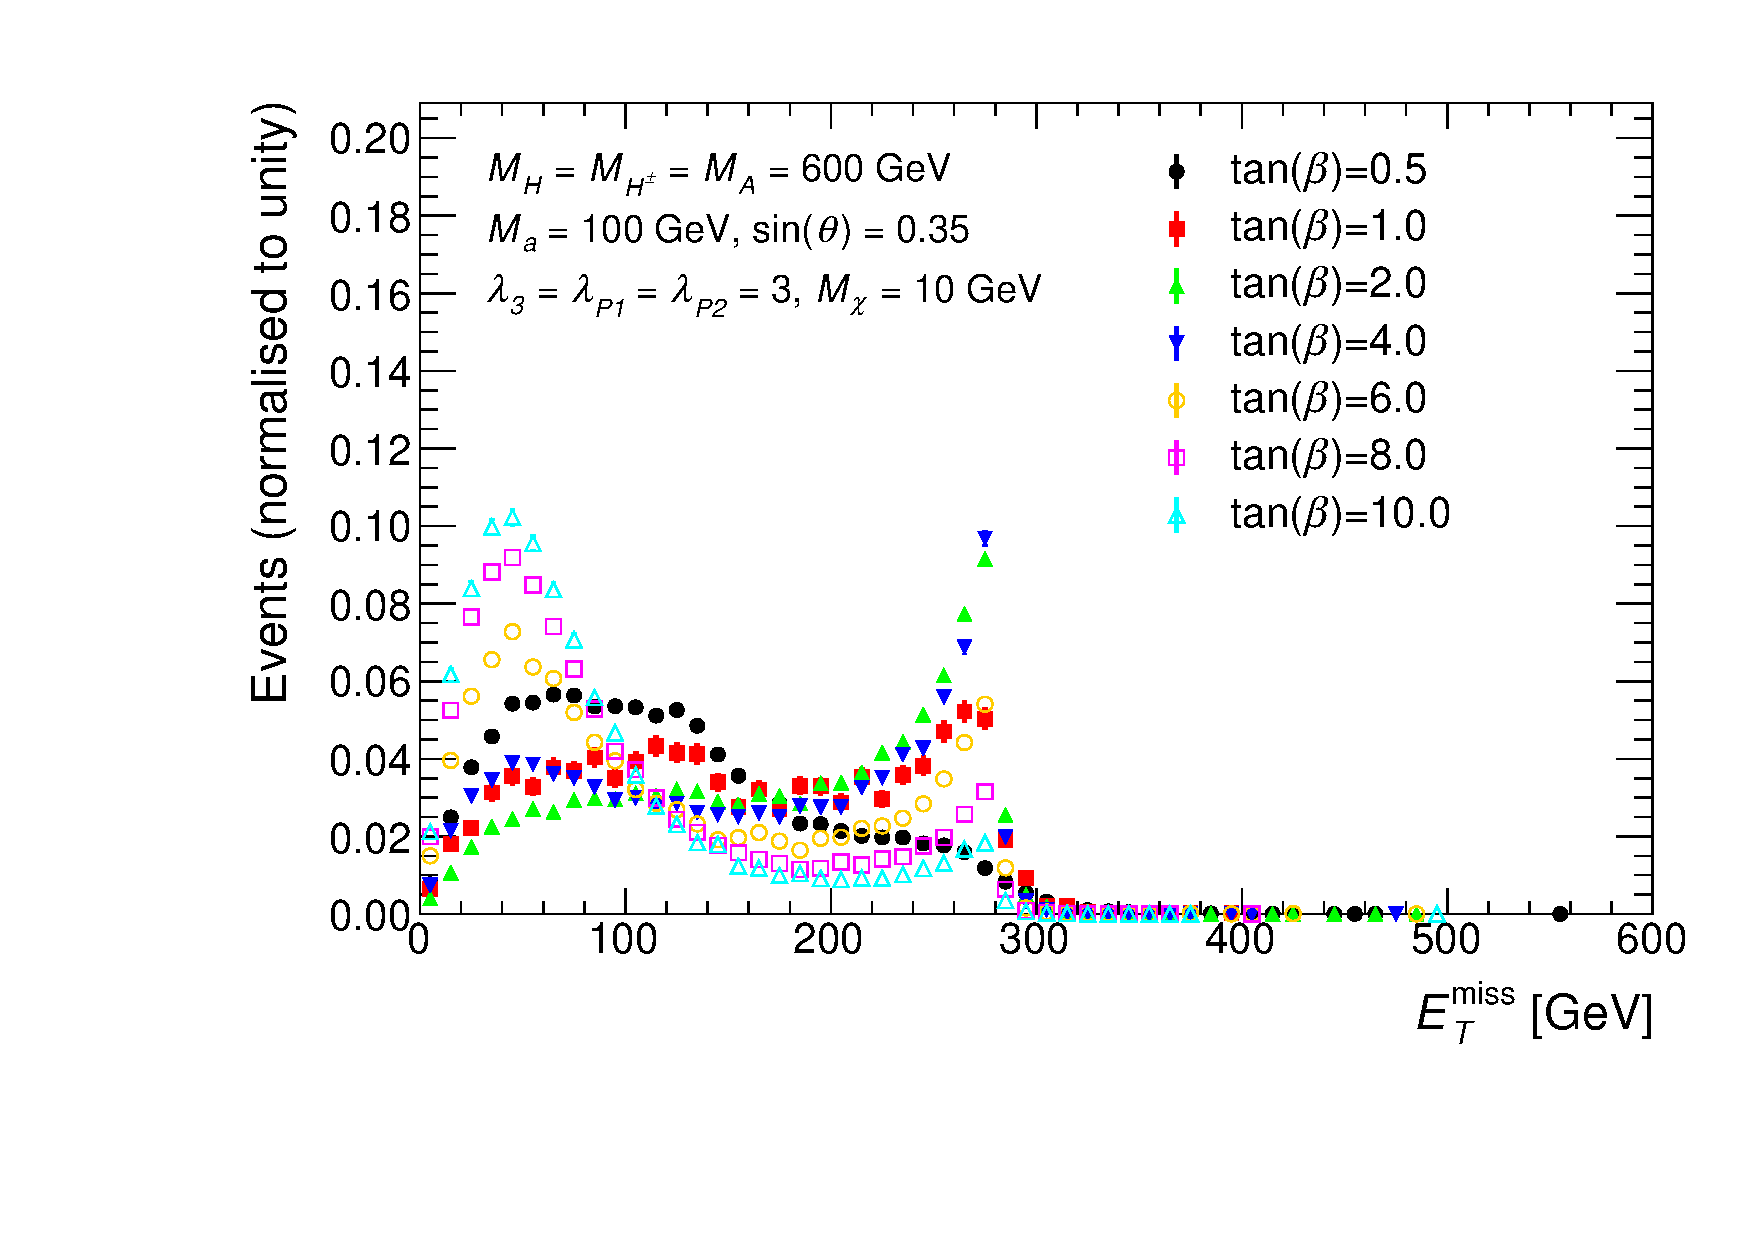
\includegraphics[width = \textwidth]{texinputs/04_grid/figures/monoHbb_tanb_scan_MA600_Ma100_MET_liny_norm2one.pdf}
\end{subfigure}
~
\begin{subfigure}{0.48\textwidth}
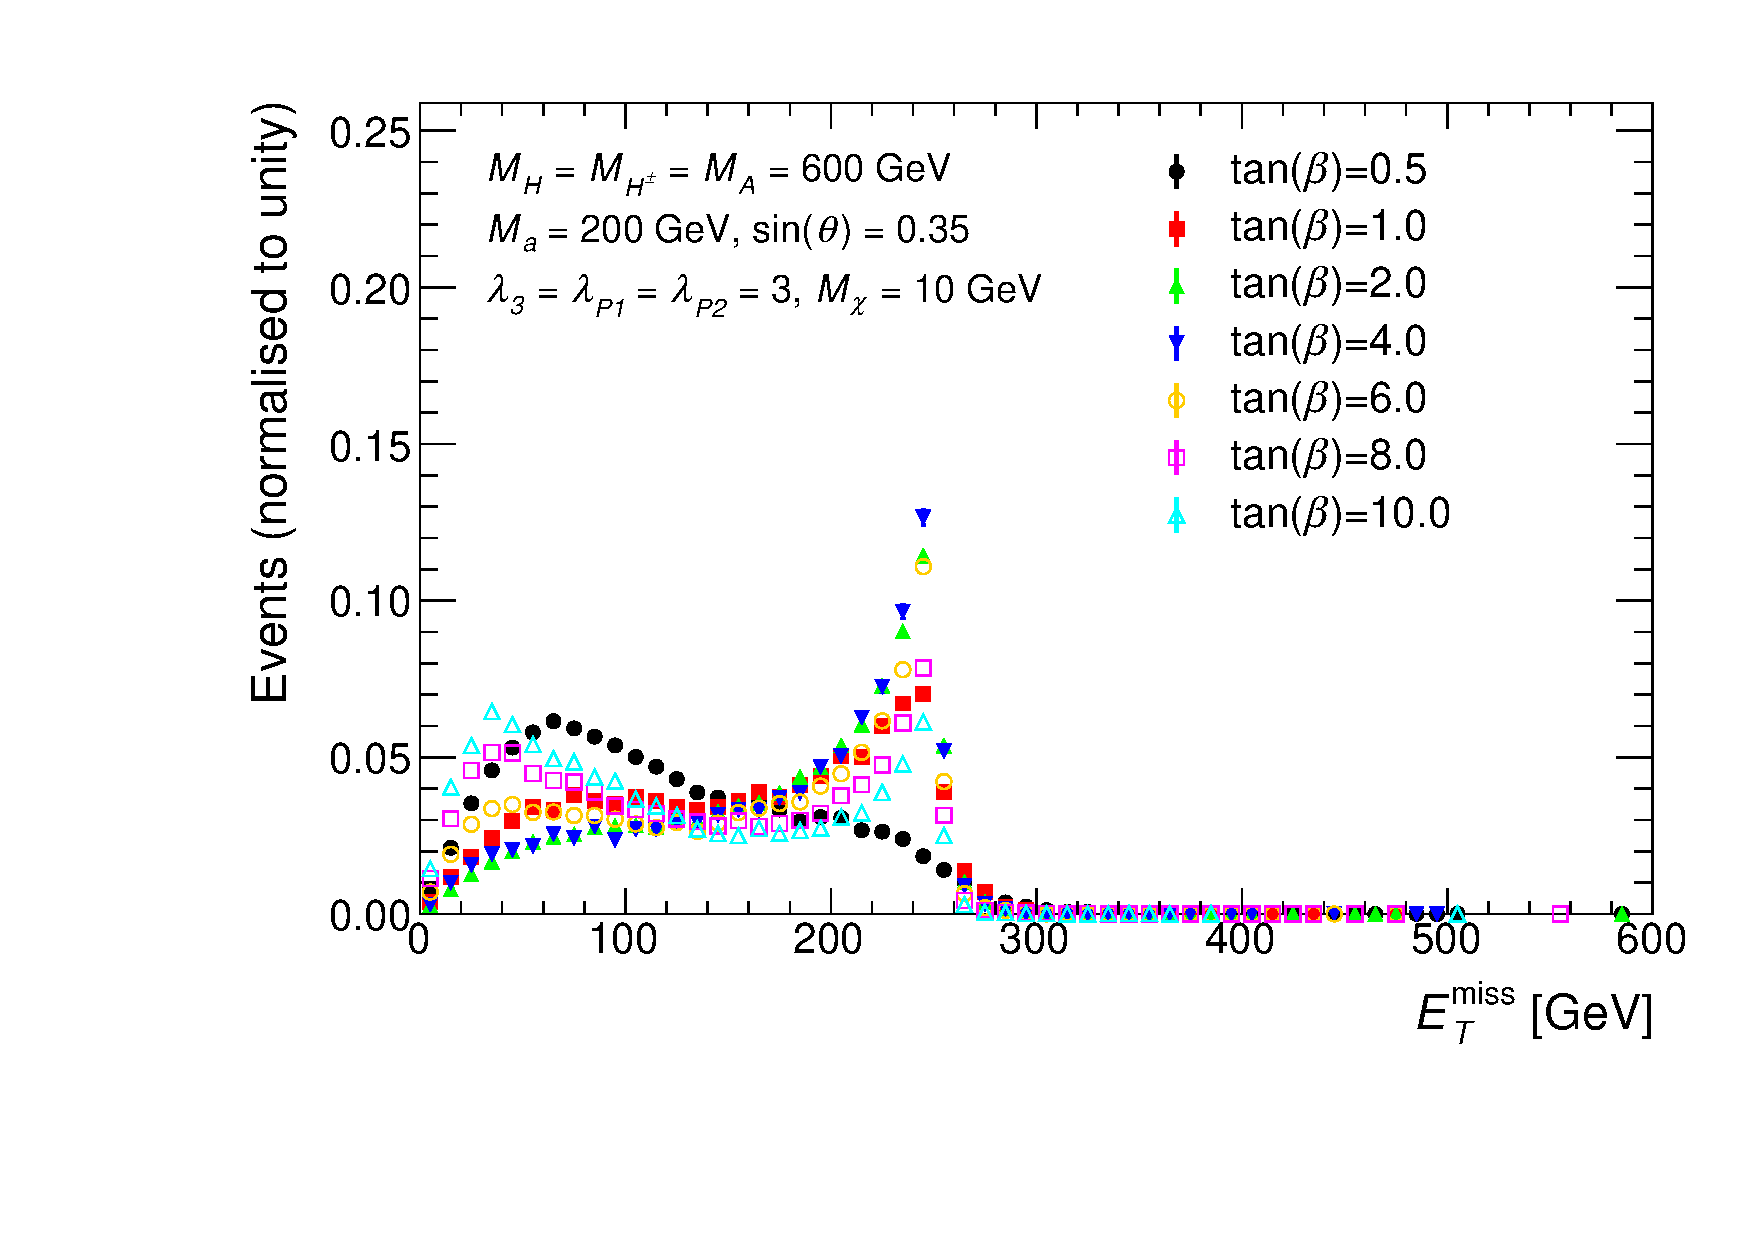
\includegraphics[width = \textwidth]{texinputs/04_grid/figures/monoHbb_tanb_scan_MA600_Ma200_MET_liny_norm2one.pdf}
\end{subfigure}
\\
\centering
\begin{subfigure}{0.48\textwidth}
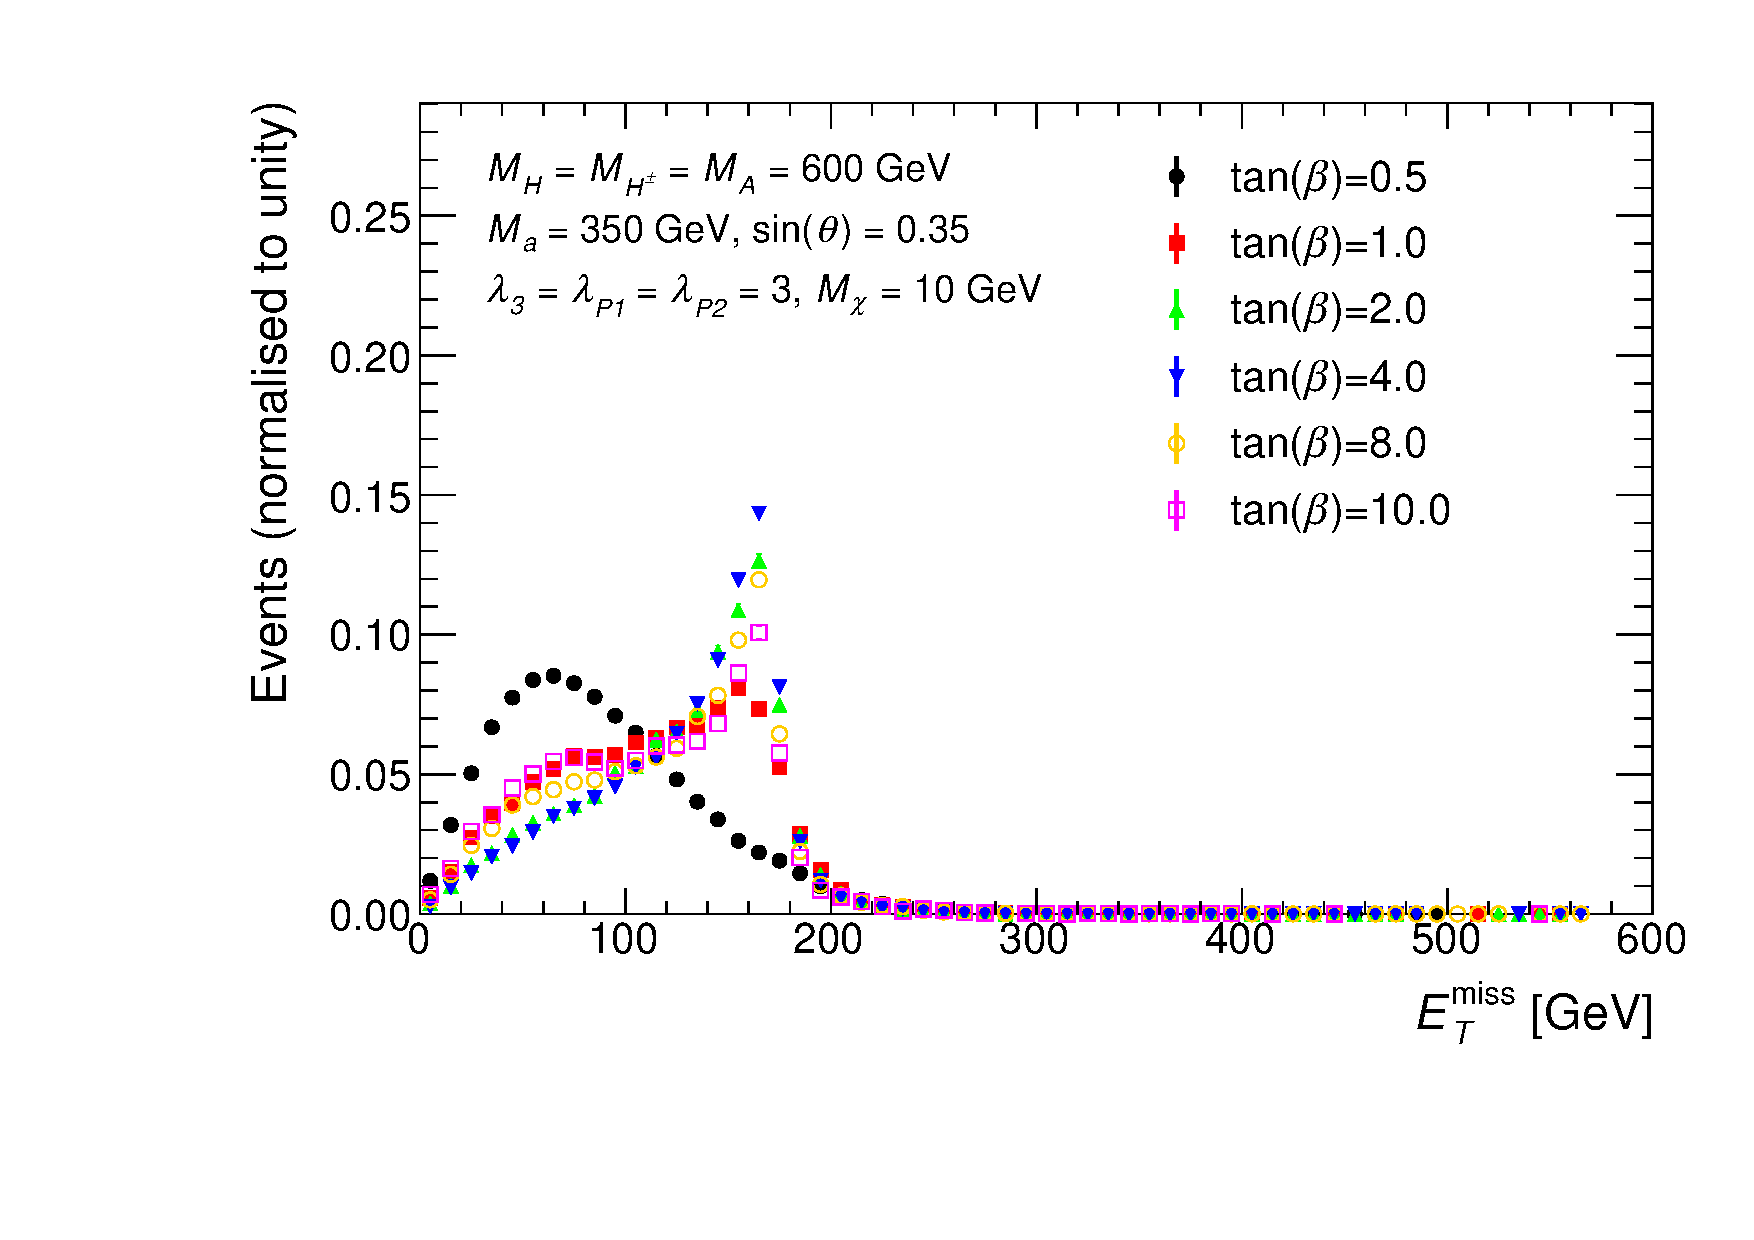
\includegraphics[width = \textwidth]{texinputs/04_grid/figures/monoHbb_tanb_scan_MA600_Ma350_MET_liny_norm2one.pdf}
\end{subfigure}
~
\begin{subfigure}{0.48\textwidth}
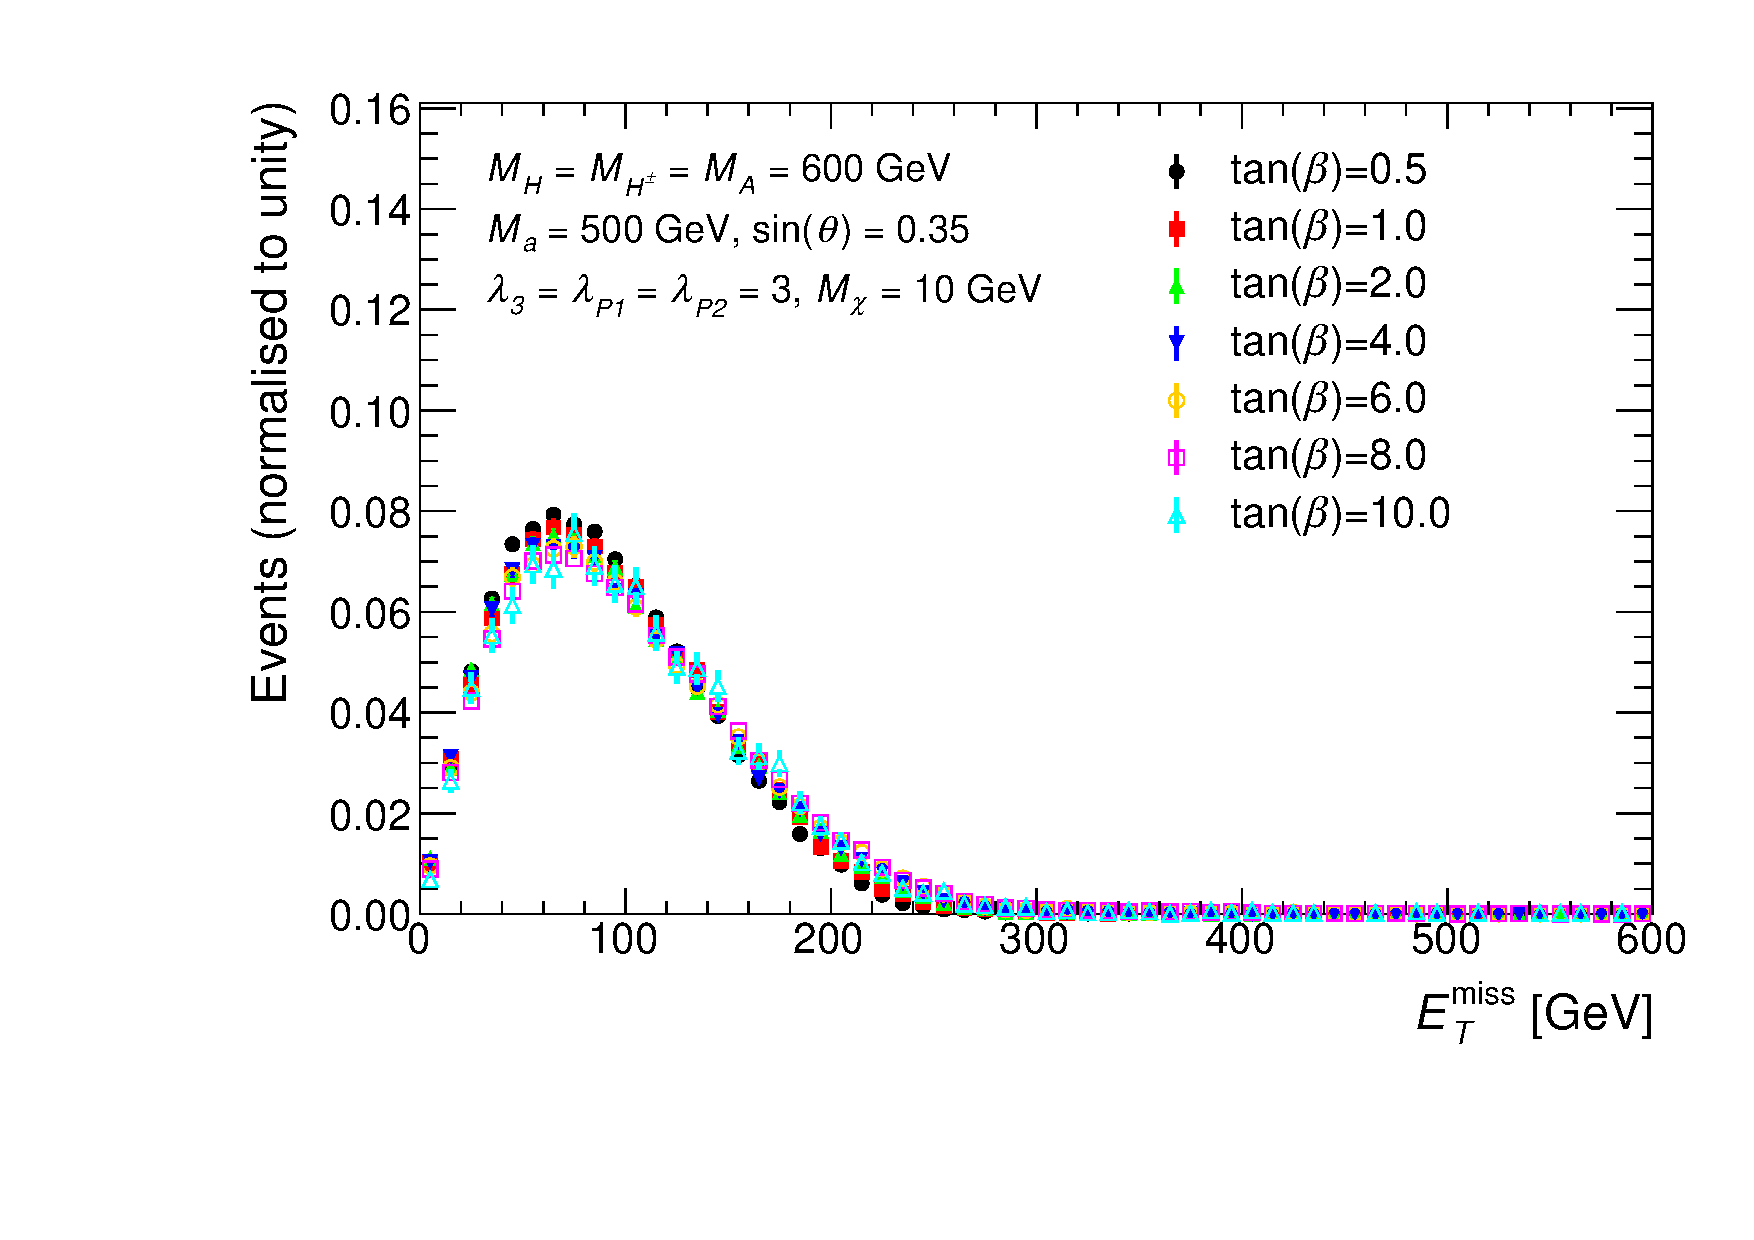
\includegraphics[width = \textwidth]{texinputs/04_grid/figures/monoHbb_tanb_scan_MA600_Ma500_MET_liny_norm2one.pdf}
\end{subfigure}
\caption[$\MET$ distribution in $h\rightarrow bb + \MET$ events for different 
$\tanb$ for $\mA = \mH = \mHc = 600 $ GeV]
{
Missing transverse momentum distribution of $h\rightarrow bb + \MET$ signal 
events at parton level with different $\tanb$ and
 fixed $\mA = \mH = \mHc = 600 $~GeV, $ \mDM = 10$~GeV, $\sinp = 0.35$, 
and $ \lap1 = \lap2 = \lam3 = 3 $. The values of $\ma$ are set to 100, 200, 
350, and 500~GeV, respectively.
The shapes of the $\MET$ distributions for different $\tanb$ are similar when 
$\mA < \mh+\ma$. Note, in these figures, both the contributions of $gg$ and $b\bar{b}$ 
initiated processes are included and a combined histogram is produced 
according to their corresponding cross sections.
}
\label{fig:monoHbb_tanb_scan_met}
\end{figure}

\begin{figure}
\centering
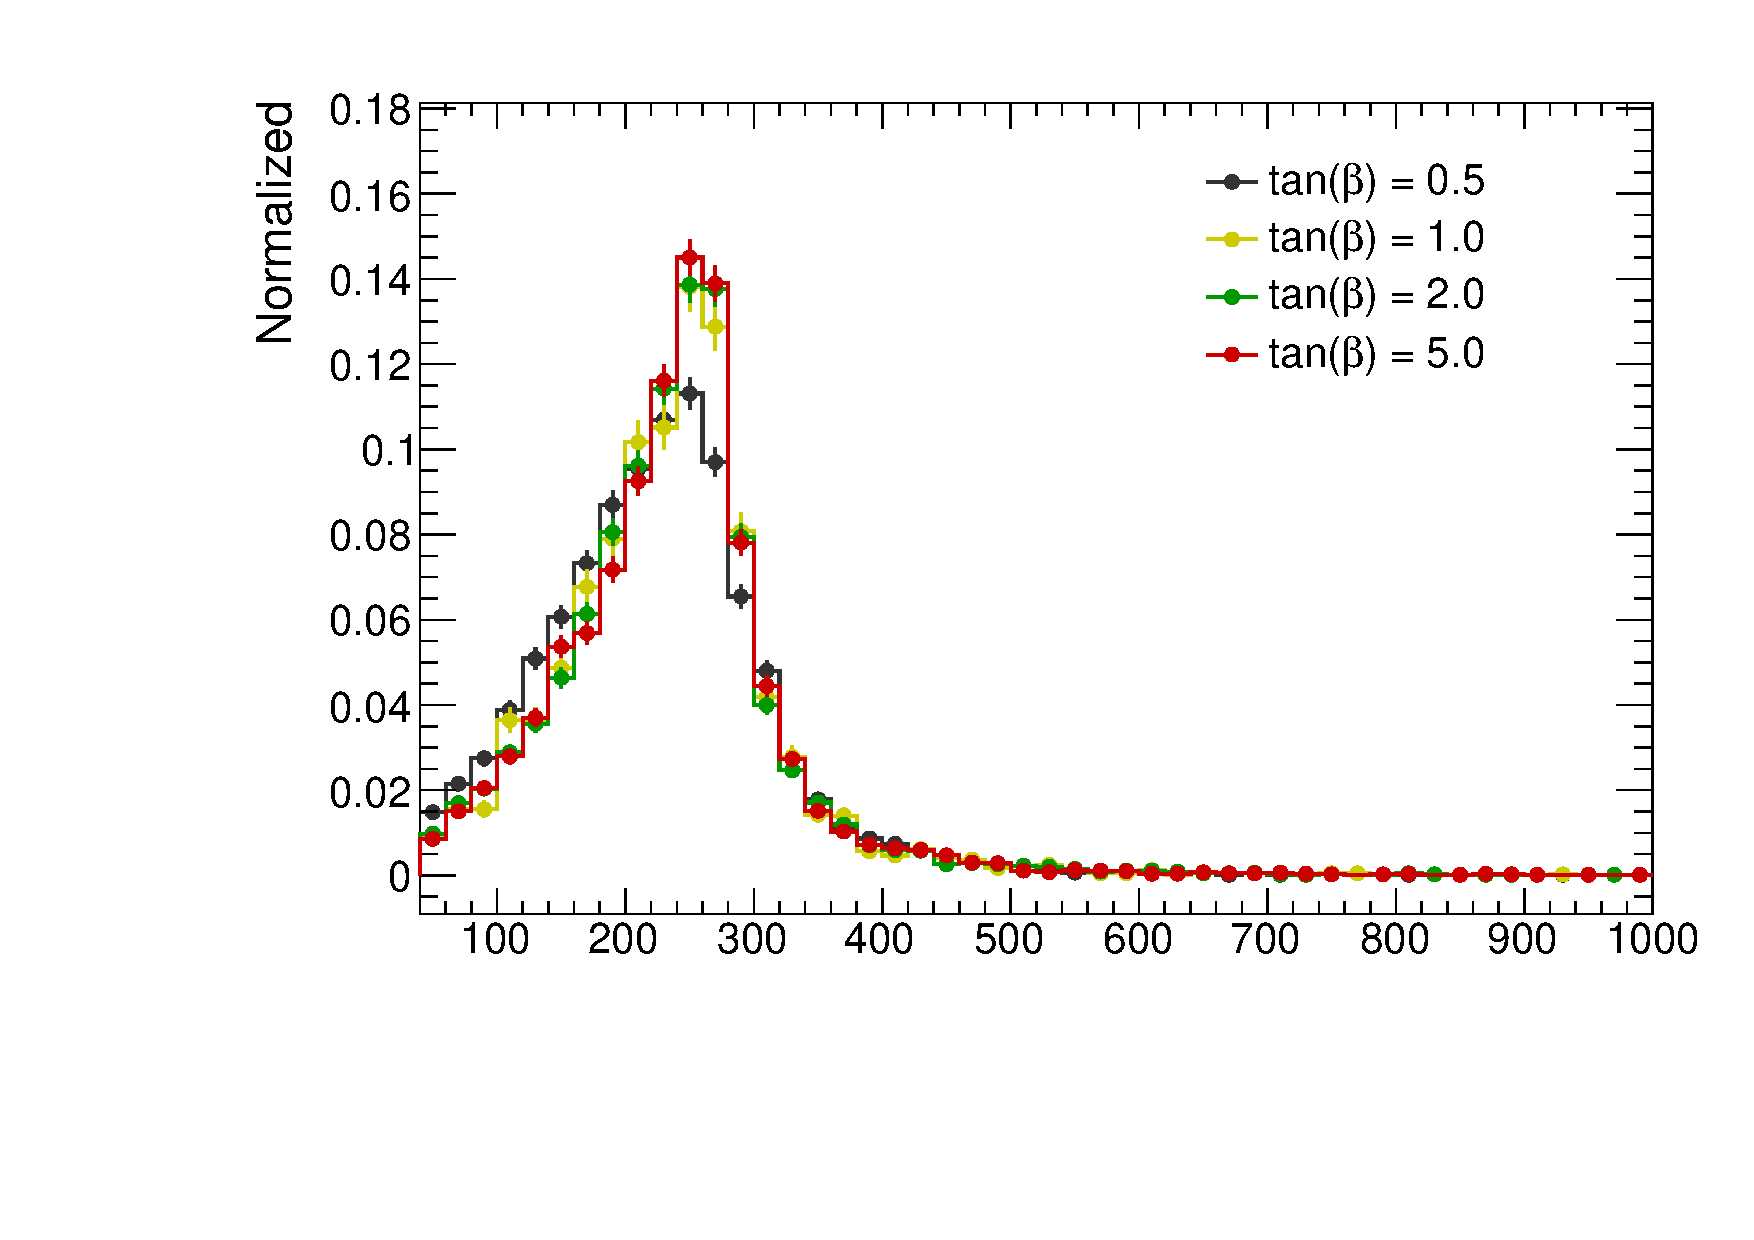
\includegraphics[width=0.48\textwidth]{texinputs/04_grid/figures/monoz/leptonic/TanbScan_mA600_ma150_MET.pdf} 
\caption{\MET distribution after preselection for scans of $\tan{\beta}$ for fixed \mA =600 \GeV and \ma = 150 \GeV. This parameter has little impact on the kinematic distributions, except for small values of \tanb where there is a slight softening and broadening of the \MET distribution caused by the increased contribution from the top box feynman diagram.}
\label{fig:monoz_kin_tanb}
\end{figure}

\subsubsection{Mass of DM fermion ($\mDM$)}

The mass of the DM fermion $\mDM$ can change the total cross section and shape of the $\MET$ distribution, depending on the mass hierarchy of the $A,a,h,\chi$ particles. This is demonstrated in \autoref{fig:monoHbb_mDM_scan_met}. 
Provided on-shell  decays $a\to\chi\chi$ are possible, i.e., $\mDM < \ma/2$, the exact value of \mDM has no effect on either kinematics or the total cross section. 
The only exception is the case $\ma/2 > \mDM > \frac{1}{2}(\ma - M_h)$. In this  $\mDM$ range, the non-resonant process $a \to h A^*\left(\chi\chi\right) $ is kinematically inaccessible. 
This reduces the overall cross section relative to the $\mDM \leq \frac{1}{2}(\ma - M_h)$ case, and slightly changes the soft part of the total $\MET$ spectrum. 
However, since the contribution of the $a \to h A^*\left(\chi \chi\right)$ process is minor in any case, the differences are negligible.

If the DM particle mass is exactly on threshold, i.e., $\mDM = \ma/2$, the total cross section is resonantly enhanced. 
This resonant threshold enhancement drops rapidly towards both higher and lower $\mDM$. Furthermore, the shape of the $\MET$ distribution at threshold, where amplitudes involving $a\to\chi\chi$ decays make up a larger fraction of the signal, differs significantly from the one below threshold. 
Below threshold ($\mDM > \ma/2$), the total cross section quickly drops by several orders of magnitude. In this regime, the shape of the $\MET$ distribution changes with $\mDM$ continuously.

\begin{figure}[tbp]
\centering
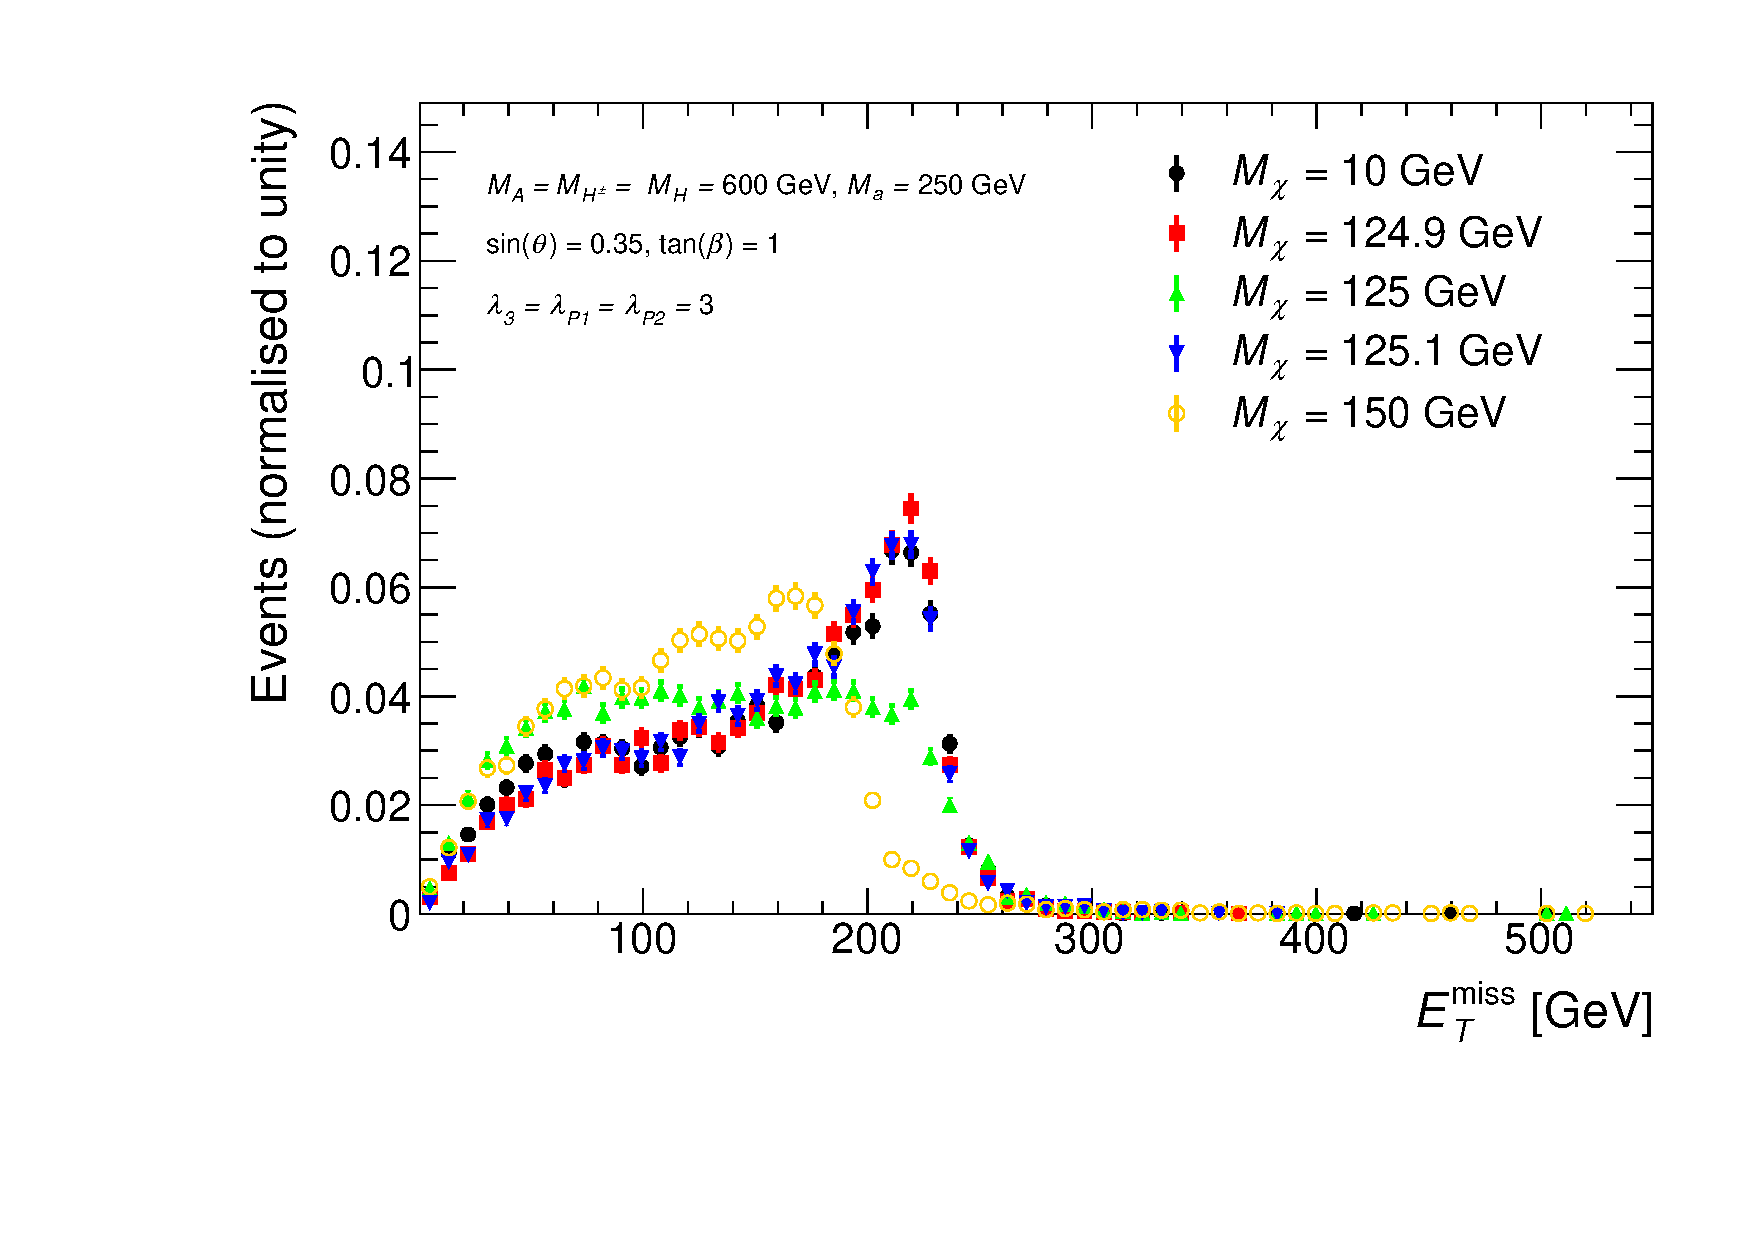
\includegraphics[width=0.7\textwidth]{texinputs/04_grid/figures/monoHbb_mDM_scan_MET_liny_norm2one.pdf}
\caption[$\MET$ distribution in \monohbb events for different $\mDM$]
{
Missing transverse momentum distribution  of \monohbb signal events at parton level for five representative models with different $\mDM$
and fixed $\mA = \mH = \mHc = 600 $ GeV $\ma = 250$ GeV, $ \sinp = 0.35, \tanb = 1$ and $ \lap1 = \lap2 = \lam3 = 3 $. 
The shape of the $\MET$ distribution does not change for $\mDM < \ma/2$, then changes significantly for $\mDM>=\ma/2$.
%
}
\label{fig:monoHbb_mDM_scan_met}
\end{figure}

Similar effects are seen in \autoref{fig:dm_scan_ll}. In the $\mDM < \frac{\ma}{2}$ region, \mDM has no effect on event yield or \MET distribution, at $\mDM = \frac{\ma}{2}$ a resonant enhancement to the cross section occurs, and in the off-shell region where  $\mDM > \frac{\ma}{2}$ cross section steeply drops.  The \MET shape remains the same up to, and even slightly above, $\mDM = \frac{\ma}{2}$, but further off shell the \MET distribution becomes increasingly disperse.  For \mDM = 200 \GeV, DM can still decay on-shell through the $A$.  For \mDM = 500 \GeV both pseudoscalars are off-shell leading to an event yield too low to fit on the figure on the left and a \MET distribution without structure.

\begin{figure}
\centering
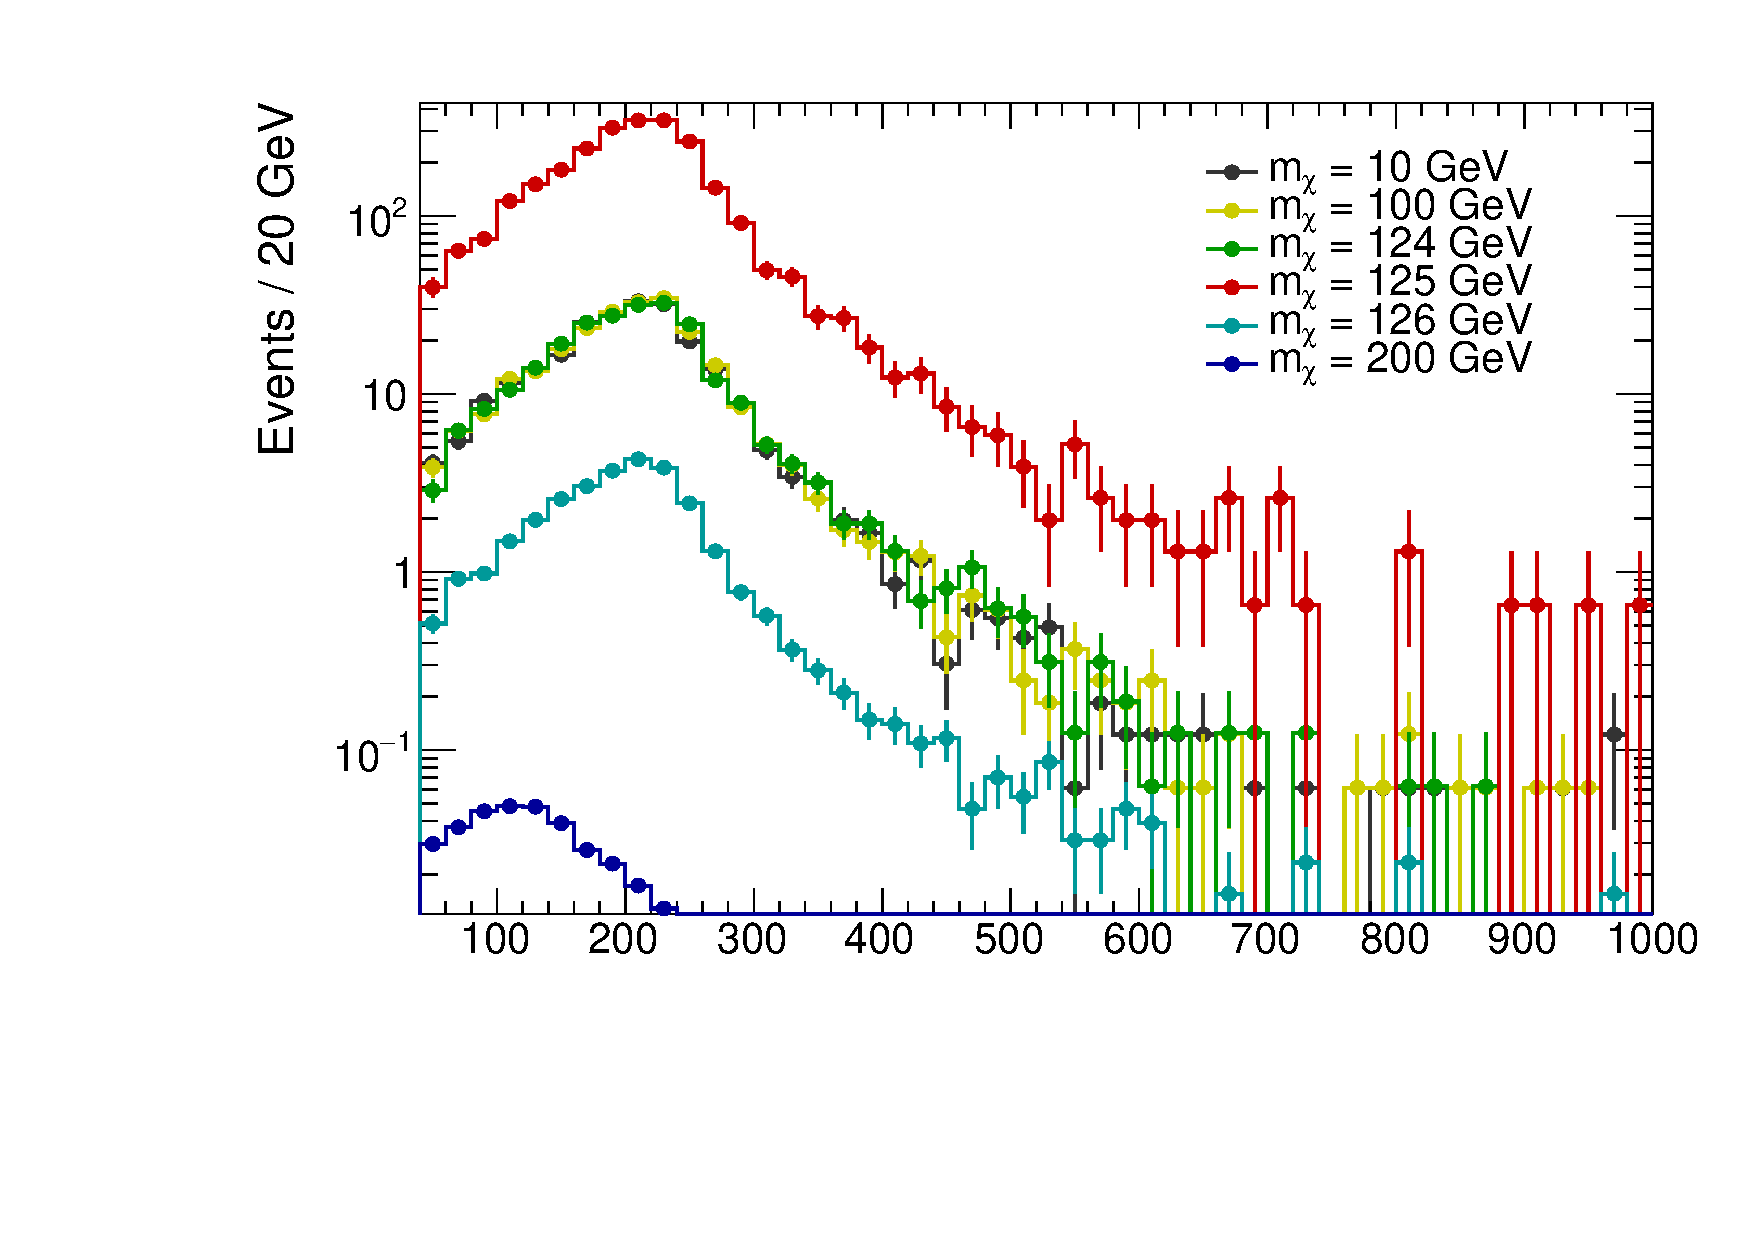
\includegraphics[width=0.48\textwidth]{texinputs/04_grid/figures/monoz/leptonic/mDMScan_mA600_ma250_MET.pdf}
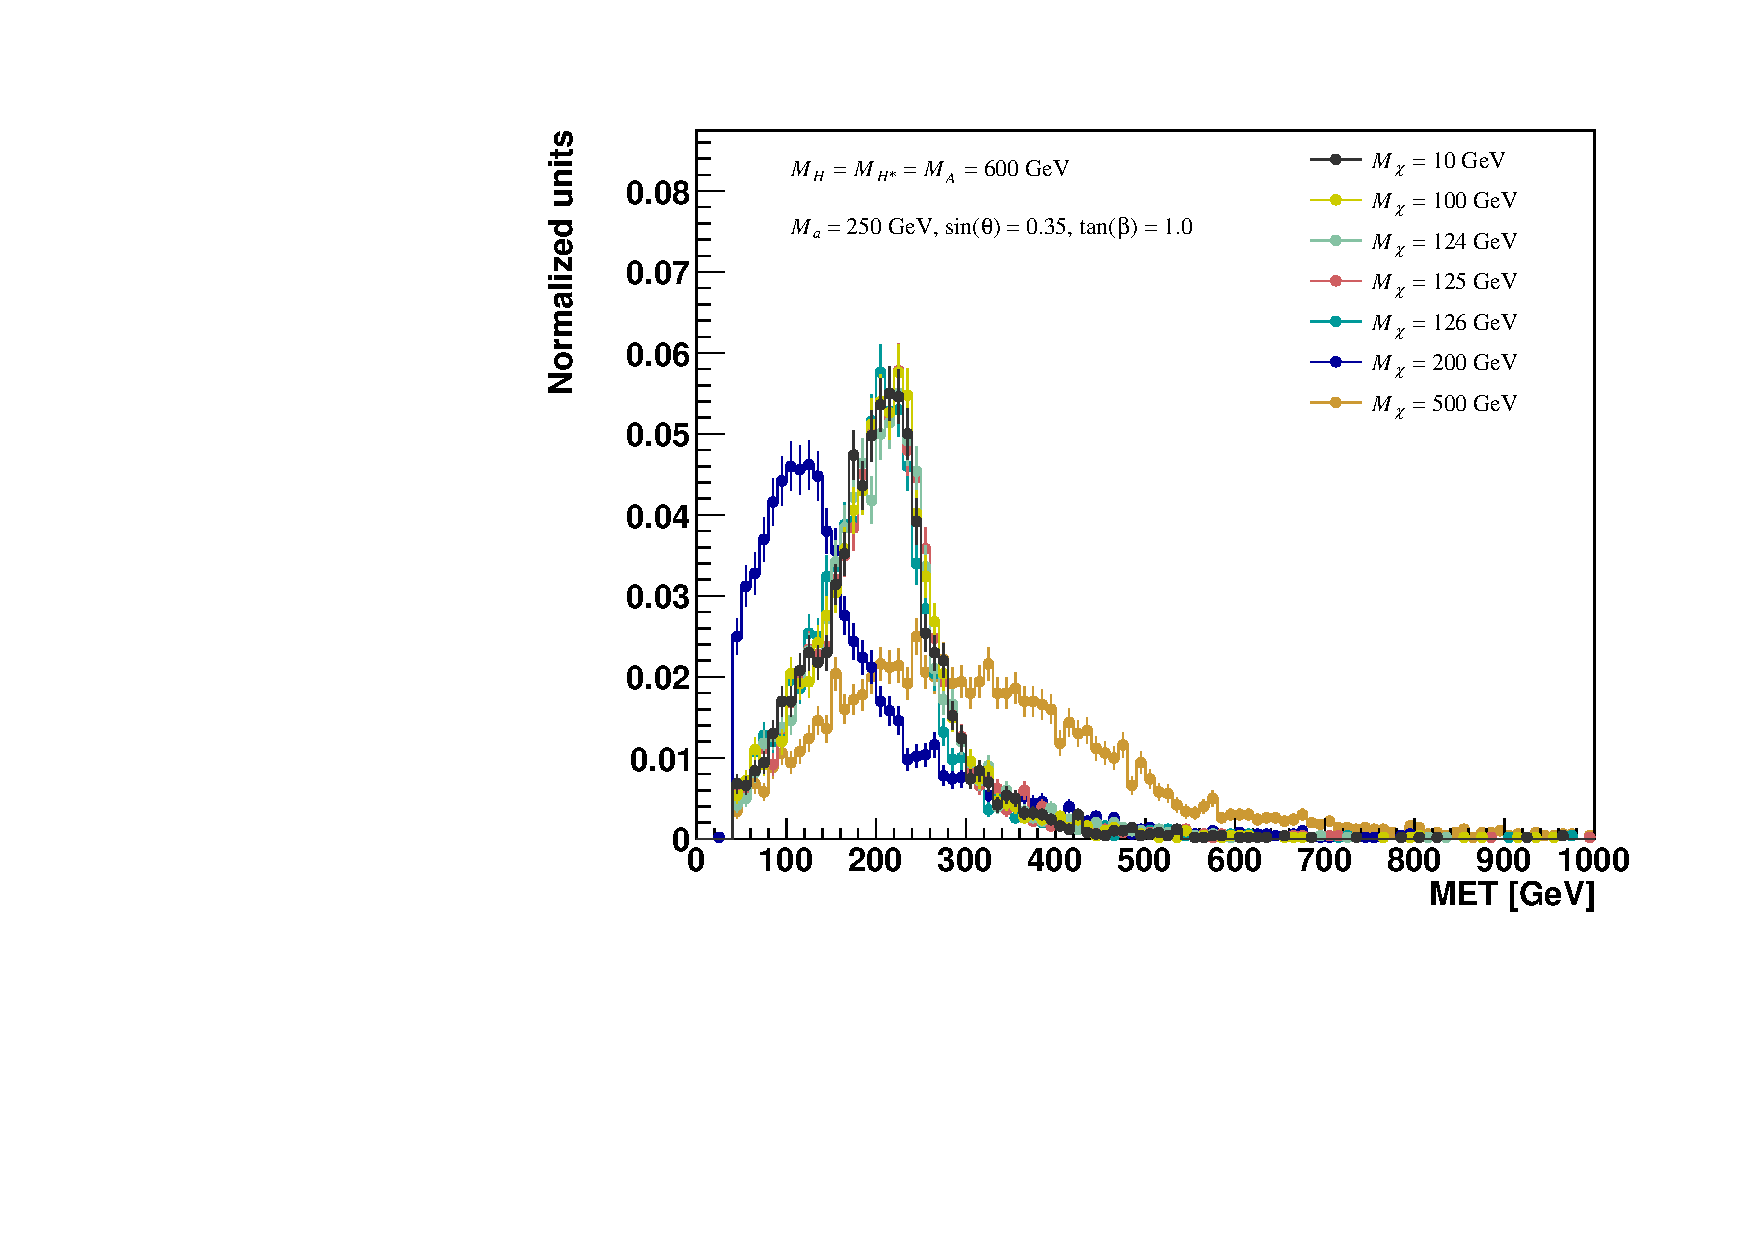
\includegraphics[width=0.47\textwidth]{texinputs/04_grid/figures/monoz/leptonic/mDMscan_ma250.pdf}
\caption{\MET distributions following preselection in the Z(lep) +\MET search are shown (left) scaled to 40 \ifb and (right) normalized to unity for different values of \mDM with fixed \mA = 600 \GeV and \ma = 250 \GeV.}
\label{fig:dm_scan_ll}
\end{figure}

A value of $\mDM$=10 is chosen for the following studies, as it produces a cross-section that is sufficiently large for this model to be detected with Run-2 LHC data and highlights the resonant features of the \MET spectrum.
%TODO: mention instability
